% !TEX root = ./guide-2e.tex
\usepackage{color}
\usepackage{url}
\usepackage{doi}
\usepackage{lmodern}
\usepackage{amsmath}
\usepackage{mathtools}
\usepackage{amsthm}
\usepackage{amssymb}
\usepackage{booktabs}
\usepackage[dvipdfmx]{graphicx}
\usepackage{listings}
\usepackage{float} 
\usepackage{placeins}
\usepackage[nameinlink]{cleveref}


%%
\title{
\jtitle{特徴量連続化によるRisk Terrain Modelingの改良}
\etitle{Risk Terrain Modeling on Continuous Features}
}
%%英文は以下を使用
%\title{Style file for manuscripts of JSAI 20XX}

\jaddress{氏名,所属,住所,電話番号,Fax番号,電子メールアドレスなど}

\author{%
\jname{橋本 響}
\ename{Kyo Hashimoto}
\and
\jname{木脇 太一}
\ename{Taichi Kiwaki}
% \and
% \jname{高知大学 理工学部 情報科学科}
% \ename{Department of Information Science, Faculty of Science and Technology, Kochi University}
}

\affiliate{
\jname{高知大学 理工学部 情報科学科}
\ename{Department of Information Science, Faculty of Science and Technology, Kochi University}
% \and
% \jname{\second{}所属和文2}
% \ename{Affiliation \#2 in English}
%\and
%\third{}Affiliation \#3 in English%%英文は左を使用
}

%%
%\Vol{28}        %% <-- 28th(変更しないでください)
%\session{0A0-00}%% <-- 講演ID(必須)

\begin{abstract}
地理的犯罪予測であるRisk Terrain Modeling(RTM)は,
廃屋や廃棄車両などの位置情報から犯罪発生リスクを算出する手法である。
しかし高い空間相関をもつRTMの予測は実際の犯罪発生の特性とは乖離しており,
不十分な予測精度として現れていた。これはRTMで離散値として構成された特徴量の問題である。
そこで本研究ではRTMの特徴量として連続量を利用することを提案した。
また併せて過去の犯罪発生に関する特徴量も追加した。
この改善により,犯罪予測と機械学習の文脈で一般的であるPAIとROC-AUCの意味において,
従来手法をそれぞれ70.7\%,13.5\%改善した. 
\end{abstract}

%\setcounter{page}{1}
\def\Style{``jsaiac.sty''}
\def\BibTeX{{\rm B\kern-.05em{\sc i\kern-.025em b}\kern-.08em%
 T\kern-.1667em\lower.7ex\hbox{E}\kern-.125emX}}
\def\JBibTeX{\leavevmode\lower .6ex\hbox{J}\kern-0.15em\BibTeX}
\def\LaTeXe{\LaTeX\kern.15em2$_{\textstyle\varepsilon}$}

\begin{document}
\maketitle

\section{はじめに}
%----------------------------------------------------------------------------
%\subsection{背景}
%------------------------------------
犯罪の防止は古今を問わず重要な社会課題である.
近年では地理情報システムの発展に伴い,
犯罪が発生した時間・場所などの各種データが蓄積されており\cite{ChicagoDataPortal},
それらに基づく犯罪予測は新たな政策提案・警察活動の指針を与えるものとして国際的に期待されている
\cite{犯罪予測}。

その代表的手法であるRisk Terrain Modeling(RTM)\cite{caplan2015risk}は,
廃屋や廃棄車両,差し押さえ物件などの位置情報(以下,地理的リスク要因)から作成した特徴量から,
近い将来における犯罪発生リスクを算出・視覚化する手法として広く利用されている\cite{地理的犯罪予測研究の潮流}。
一般的にRTMでは,地理的特徴量は前処理を経て離散的なカテゴリデータへ変換され,線型モデルへ入力される\cite{犯罪予測, caplan2015risk}。
政策立案者や治安維持機関は,RTMによりリスクの高いエリアを特定し,防犯資源の効率的な配分に役立てる事ができる\cite{犯罪予測}。

%------------------------------------
%\subsection{研究目的}
%\subsection{従来手法の課題}\label{conv_limit:sec}
%------------------------------------
%基盤となる統計モデルは主に線形モデルとして構築されてきた。
従来のRTMにより算出された犯罪リスク値は,実際のデータの特性と乖離した,異常に高い空間相関を持つ。
この特異な振る舞いは不十分な予測精度として現れていた。
この問題点は,特徴量の離散化の結果,従来のRTMにおいて予測変数に含まれる情報が過度に制限されることに起因していた。
そこで本研究では,離散化を省き,連続的特徴量に対するRTMを提案する。
この改善により情報の損失を抑え,リスク予測結果を実際の犯罪分布に近づけることを実現した。
%また定量的な評価としては,犯罪予測の文脈で広く利用されるされる。 
更に地理的リスク要因と並列に犯罪発生情報を予測変数として導入し,更なる予測精度を向上を実現した。

\section{関連研究}
\label{chapter_2}
%----------------------------------------------------------------------------
\subsection{RTMの実装}
\label{conv_imp:sec}
%------------------------------------
RTM\cite{caplan2015risk}は,
対象地域を特定幅のグリッドで小区画(以下,グリッドセル)へ分割し,各グリッドセルで犯罪発生リスクを予測する。
まず応答変数は,各グリッドセルでの特定種類(e.g., 強盗)の犯罪発生件数である。
予測変数は,地理的リスク要因から生成した離散的特徴量であり,
対象グリッドセル付近におけるリスク要因の空間分布を反映する,以下の2種の特徴量から構成される。

まず一つ目の特稜々はグリッドセル中心に最も近接する地理的リスク要因との距離に関する特徴量であり,
具体的には距離を2水準(0:基準距離外,1:基準距離内)へ離散化したものである。

二つ目の特徴量は,地理的リスク要因に対するカーネル密度推定から構成される。
まずそれぞれの地理的要因について特定のスケールパラメータでカーネル密度推定を実行する\cite{bishop}。
そしてグリッドセル中心点における確率密度推定値を2水準(0:平均+2標準偏差未満,1:平均+2標準偏差以上)に離散化する。

一つ目の方法における基準距離および二つ目の方法におけるスケールパラメータはRTMのハイパーパラメータである。
これらを適切に設定することで,グリッドセル付近の地理的リスク要因をモデリングする際の実効的なスケールを調節することが出来る。
またこれらのハイパーパラメータは複数の値を設定し,それぞれで独立に特徴量を構成して,モデルへ並列に組み込むこともできる。

これらの応答変数と予測変数に対して,ポアソン回帰\cite{poisson}もしくは負の二項回帰\cite{Hilbe_2011}を実行する。
更にステップワイズ法\cite{islp}によるBayesian information criteria最小化を通じて変数選択を行い,重要なリスク要因の判定が行われる。
学習後のモデル予測値は犯罪発生リスクとして利用し,それを地図上へヒートマップとして表示したものがリスクマップである。

% % ポアソン回帰 (Poisson Regression)
% \begin{align}\label{poisson}
%    Y_i \sim \text{Poisson}(\lambda_i) \text{,}
%    \log(\lambda_i) = X_i \beta 
%  \end{align}
 
%  % 負の二項回帰 (Negative Binomial Regression)
%  \begin{align}\label{negative binominal}
%    Y_i \sim \text{NB}(\mu_i, \theta) \text{,}
%    \log(\mu_i) = X_i \beta 
%  \end{align}
 
%  この手法では,地理的リスク要因による特徴量を離散的なカテゴリデータとして表現している。
%  例えば,各グリッドセルが特定の地理的リスク要因から,
%  一定距離内に存在するか否かを$0$または$1$で表す。

%------------------------------------
\subsection{予測精度向上への取り組み}
%------------------------------------
% 大山ら\cite{大山智也2020短期的}は,最新の犯罪発生に伴う短期的なリスクと,
% RTMの予測因子では捉えきれない長期的なリスクを組み合わせることで,RTMを発展させた。
% この改善により,既存のRTMを上回る予測精度と安定性を得た。
% このことは,地理的リスク要因以外の環境要因や再犯リスクを考慮することで,
% どの時期でも安定した予測が可能になることを示唆している。
大山\cite{大山智也2020日本}は,RTMに対して犯罪発生情報を組み合わせることで,
中長期的な潜在リスクに加えて,短期的な顕在リスクも算出するモデルを構築した。
この改善により,的中率においてはRTMをを上回る予測精度を得たが,predictive accuracy index(PAI)はRTMを下回る結果となった。

%----------------------------------------------------------------------------
\section{提案手法:連続RTM}
\label{chapter_3}
%----------------------------------------------------------------------------
RTMの特徴量構成法は離散化により予測変数の情報が十分にモデルへ伝わらず,結果としてモデルが未学習となる可能性がある。
また\citet{caplan2015risk}のRTM実装は古典的なステップワイズ法\cite{islp}による変数選択に依存するが,同等の効果はより効率的なLasso回帰\cite{Lasso}でも実現できる。これら点から,本研究では以下へ取り組む:
\begin{enumerate}
  \item 未学習防止のための連続型特徴量導入,
  \item Power transformとLasso回帰によるモデル構成。
\end{enumerate}
この改善によるモデルを連続RTMとする(単にRTMと書いた時は\citet{caplan2015risk}による元々の実装を指すとする)。

また\cref{conv_imp:sec}

並列に応答変数以外の犯罪発生情報を予測に用いる手法について述べる。
また同時にRTM\cite{caplan2015risk}を再実装する。

%------------------------------------
\subsection{連続型特徴量(Continuous features, CF)}
%------------------------------------
従来手法\cite{caplan2015risk}では,距離とカーネル密度推定値による連続型特徴量を離散化するが,
CFでは離散化せず連続型特徴量のままRTMの予測変数とする。
%------------------------------------
\subsection{犯罪特徴量を追加した連続化(Continuous  Features Including Crime Features, CI)}
%------------------------------------
従来手法\cite{caplan2015risk}では,応答変数以外の犯罪発生情報を予測に用いていなかった。
犯罪発生情報を予測に取り入れる手法は先行研究\cite{大山智也2020日本}でも提案されているが,
予測精度が向上したとはいえない。
そこでCIではCFの発展として,応答変数以外の犯罪発生情報を連続型特徴量としてRTMの予測変数とする。
%------------------------------------
\subsection{RTMの実装}
%------------------------------------
本研究では前処理として,応答変数と予測変数の分布をYeo-Johnson変換\cite{weisberg2001yeo}
により正規分布に近づける。
なおYeo-Johnson変換は逆変換が可能である。
式(\ref{yeo})にYeo-Johnson変換の詳細を示す。
\begin{equation}\label{yeo}
   x^{(\lambda)} =
   \begin{cases} 
   \frac{(x+1)^\lambda - 1}{\lambda}, & \text{if } \lambda \neq 0, x \geq 0 \\ 
   \log(x+1), & \text{if } \lambda = 0, x \geq 0 \\ 
   \frac{-(-x+1)^{2-\lambda} + 1}{2-\lambda}, & \text{if } \lambda \neq 2, x < 0 \\ 
   -\log(-x+1), & \text{if } \lambda = 2, x < 0
   \end{cases}
\end{equation}
なお,$x$は変換前のデータ,$x^{(\lambda)}$は変換後の値,$\lambda$は変換パラメータを表す。
その後,Lasso回帰分析を用いて変数選択を行い,回帰係数を推定する。
また,交差検証により最適な正則化パラメータを決定する。

モデルの出力値に対して,前処理で実行したYeo-Johnson変換の逆変換を行って,
予測値の分布を元の犯罪の分布に近づけた。モデルの予測値は連続値であるため,
精度評価やリスクマップ表示の際には,予測値をそれぞれを適切な基準で離散化する。
%----------------------------------------------------------------------------
\section{実験}
%----------------------------------------------------------------------------
従来手法\cite{caplan2015risk}による,距離とカーネル密度推定値\cite{bishop2007}による離散型特徴量を
予測変数とするモデルをDF(Discrete features)とする。
%------------------------------------
\subsection{データセット}
%------------------------------------
本研究では,\cite{caplan2015risk}が提案するRTMと同様に,
アメリカ合衆国のイリノイ州クック郡の郡庁所在地であるシカゴ市を対象領域とする.
応答変数を構成する犯罪発生地点及び,予測変数を構成する地理的リスク要因の位置情報は,
\cite{ChicagoDataPortal}のAPIを用いて緯度経度情報として取得した.

取得したデータ期間は2011年1月1日〜2014年12月31日で,
それぞれの犯罪発生地点と地理的リスク要因の位置情報は,
ともに発生時刻・記録年を基に1年単位で取得した.
表\ref{tab:2011-2014-data}に取得した全データ件数を示す.

\begin{table}
  \centering
  \caption{2011年から2014年のデータ}
  \label{tab:2011-2014-data}
  \begin{tabular}{lrrrr}
  \toprule
  カテゴリ & 2011 & 2012 & 2013 & 2014 \\
  \midrule
  強盗 & 26577 & 22783 & 17854 & 14490 \\
  \midrule
  廃墟 & 15365 & 11971 & 8363 & 5446 \\
  放置車両 & 19907 & 17390 & 16077 & 20358 \\
  路地灯消灯 & 46697 & 19944 & 15177 & 21684 \\
  街灯消灯 & 33895 & 30893 & 22650 & 64857 \\
  学校 & 674 & 681 & 672 & 680 \\
  差し押さえ物件 & 16680 & 16120 & 11131 & 7511 \\
  落書き除去 & 136873 & 109908 & 137058 & 124721 \\
  不衛生な場所 & 17888 & 19088 & 18029 & 18997 \\
  \midrule
  暴行 & 60306 & 58998 & 53887 & 49230 \\
  器物損壊 & 37234 & 35771 & 30779 & 27637 \\
  窃盗 & 74770 & 75170 & 71270 & 61127 \\
  性的暴行 & 1402 & 1347 & 1197 & 1216 \\
  売春 & 2424 & 2200 & 1652 & 1608 \\
  賭博 & 736 & 724 & 596 & 393 \\
  酒類法違反 & 619 & 573 & 464 & 394 \\
  武器違反 & 3879 & 3904 & 3240 & 3099 \\
  誘拐 & 266 & 234 & 242 & 217 \\
  公務執行妨害 & 1041 & 1227 & 1277 & 1393 \\
  傷害 & 20343 & 19848 & 17920 & 16830 \\
  殺人 & 437 & 515 & 431 & 428 \\
  性犯罪 & 1053 & 1035 & 1004 & 909 \\
  詐欺行為 & 12329 & 13239 & 13215 & 14788 \\
  自動車盗難 & 19353 & 16450 & 12552 & 9846 \\
  薬物犯罪 & 38527 & 35417 & 34057 & 28836 \\
  放火 & 504 & 469 & 363 & 394 \\
  脅迫 & 171 & 156 & 133 & 114 \\
  児童関連犯罪 & 2281 & 2190 & 2319 & 2304 \\
  不法侵入 & 8634 & 8197 & 8122 & 7500 \\
  ストーカー行為 & 181 & 206 & 153 & 140 \\
  治安妨害 & 3089 & 3001 & 3131 & 2896 \\
  その他の犯罪 & 20134 & 17471 & 17979 & 16902 \\
  \bottomrule
  \end{tabular}
  \end{table}

%------------------------------------
\subsection{RTMの実装条件}
%------------------------------------
分析にあたっては,対象地域に130m×130mのグリッドセルを設定し,
各グリッドセルでの犯罪発生リスクを予測する。
応答変数は各グリッドセルで発生した強盗犯罪件数,
予測変数は地理的リスク要因から生成した特徴量である。

取得したデータは,地理的座標系に基づいており,緯度経度情報として提供されているが,
本研究では距離計算や空間分析を正確に行うため,PythonのGeoPandas\cite{geopandas}を使用し,
メートル単位での解析が可能な平面直角座標系(EPSG:26971)に変換した。
また,データ品質を保証するため,明らかに誤った位置情報(NaN,0,etc.)と
シカゴ市領域外の位置情報は事前に除外した。

取得したデータに対する前処理におけるPowerTransformのYeo-Johnson変換の実装には,
sklearn.preprocessing.PowerTransformer\cite{scikit-learn}を用いた。
なお,Yeo-Johnson変換と同時に応答変数と予測変数の標準化も実施した。

また最適な正則化パラメータは,20foldの交差検証\cite{islp}で探索した。
実装には,sklearn.linear\_model.LassoCV\cite{scikit-learn}を用いた。
%------------------------------------
\subsection{評価方法}
%------------------------------------
モデルが予測した犯罪発生リスクを,
高リスク($平均+1標準偏差以上$)と低リスク($平均+1標準偏差未満$)にカテゴリー化する。
各手法の予測精度は,犯罪予測の文脈で一般的な
的中率\cite{joshi2020considerationsdevelopingpredictivemodels}と
PAI(Predictive Accuracy Index)\cite{chainey2008utility}と
ROC-AUC\cite{islp}の3つの指標で年単位の評価を行う。

的中率とは,予測モデルが「高リスク」と特定したエリアの中で、実際に犯罪が発生した割合である。
(\ref{hitrate})式に的中率の計算式を示す。

\begin{equation}\label{hitrate}
  的中率=\frac{高リスク判定エリア内の犯罪数}{全エリアの犯罪数}
\end{equation}

的中率では,低リスクエリアを高リスクエリアと誤識別する偽陽性(False Positive)を
評価できない。そのため的中率を最大とするモデルは,
高リスクエリアが広がりすぎて実用上の有用性が下がる可能性があるため,
これに加えて\cite{chainey2008utility}が考案したPAI(Predictive Accuracy Index)を評価に用いる。

PAIとは,高リスクエリア内で発生した犯罪の割合を、そのエリアの全体に占める面積割合で割った値である。
PAIが高いほど、モデルの予測精度が高いとされる。
(\ref{pai})式に的中率の計算式を示す。

\begin{equation}\label{pai}
  PAI=\frac{的中率}{\frac{高リスクエリア面積}{全エリア面積}}
\end{equation}
PAIと同様にROC-AUCも偽陽性を評価する。
% ROC(Receiver Operating Characteristic)曲線とは,
% 機械学習モデルの分類性能を評価するための代表的な手法の1つである。
% ROC曲線は,分類モデルの予測スコアに対して異なる閾値を設定し,
% それに応じた真陽性率(True Positive Rate, TPR)と
% 偽陽性率(False Positive Rate, FPR)をプロットすることで得られる。
% 曲線の下の面積がAUC(Area Under the Curve)と呼ばれ,
% モデルの識別能力を定量的に表す指標として用いられる.
% AUCは0.5から1.0の範囲を取り,この値が大きいほどモデルの分類性能が優れていることを意味する。

\subsection{実験条件}
%------------------------------------
学習データとテストデータの構成を,1年ずつ予測変数と応答変数の対をずらすことで,予測に未来の情報を用いないようにする。
学習データの構成は,2011年の地理的リスク要因を予測変数としてそれに対する応答変数を2012年に発生した強盗犯罪とする。
これに加えて,2012年の地理的リスク要因を予測変数として,それに対する応答変数を2012年に発生した強盗犯罪とする。
この計2年分の予測変数と応答変数の対を学習データとする。
またテストデータは,2013年の地理的リスク要因を予測変数としてそれに対する応答変数を2014年に発生した強盗犯罪とする。

DF,CFの応答変数は,各グリッドセル内で発生した強盗犯罪件数である。
また予測変数として用いた地理的リスク要因は,
廃屋,放置車両,路地灯消灯,街灯消灯,学校,差し押さえ物件,落書き除去,不衛生な場所
の8つである。(表\ref{tab:2011-2014-data})

CIの応答変数は,各グリッドセル内で発生した強盗犯罪件数である。
また予測変数として用いた地理的リスク要因は,
廃屋,放置車両,路地灯消灯,街灯消灯,学校,差し押さえ物件,落書き除去,不衛生な場所
の8つと強盗以外の犯罪種の24種である。(表\ref{tab:2011-2014-data})

なお,従来手法による離散型特徴量(DF)の構成に用いた,特定の距離とバンド幅とは271m,591m,779m,1003mである。
これらの距離はシカゴ市の2ブロック,4ブロック,6ブロック,8ブロックに相当する。
%------------------------------------
\subsection{結果}
%------------------------------------



% \ref{non-crime-no-timeseries-result}同様に予測結果を示す.

2014年に実際に起った強盗犯罪の発生地点に基づいた実際のリスクマップを
図\ref{fig:non-crime-timeseries-actual-risk}に示す.
DFによるリスクマップを図\ref{fig:non-crime-timeseries-df-risk}に,
CFによるリスクマップを図\ref{fig:non-crime-timeseries-cf-risk}に,
CIによるリスクマップを図\ref{fig:non-crime-timeseries-ci-risk}に
% NEによるリスクマップを図\ref{fig:non-crime-timeseries-ne-risk}に,
% LDによるリスクマップを図\ref{fig:non-crime-timeseries-ld-risk}に,
% GFによるリスクマップを図\ref{fig:non-crime-timeseries-gf-risk}に,
% TGによるリスクマップを図\ref{fig:non-crime-timeseries-tg-risk}に,
% GF+TGによるリスクマップを図\ref{fig:non-crime-timeseries-gf-tg-risk}
示す.
% \ref{non-crime-no-timeseries-result}同様に,
実際のリスクマップと比べて,離散型特徴量(DF)によるリスクマップでは高い空間相関を持つが,
連続型特徴量(CF)と犯罪込み連続型特徴量(CI)によるリスクマップは空間相関が削減された.


% また,
% 4カテゴリーの混同行列を図\ref{fig:non-crime-timeseries-4cm}に,
% 2カテゴリーの混同行列を図\ref{fig:non-crime-timeseries-2cm}に,
% 各モデルによるFP・FNのグリッドセルを
% 図\ref{fig:non-crime-timeseries-df-fnp}から
% 図\ref{fig:non-crime-timeseries-gf-tg-fnp}に示した.

%------------------------------------------
% risk map
%------------------------------------------



% \begin{figure}
%   \centering % 図を中央寄せにする
%   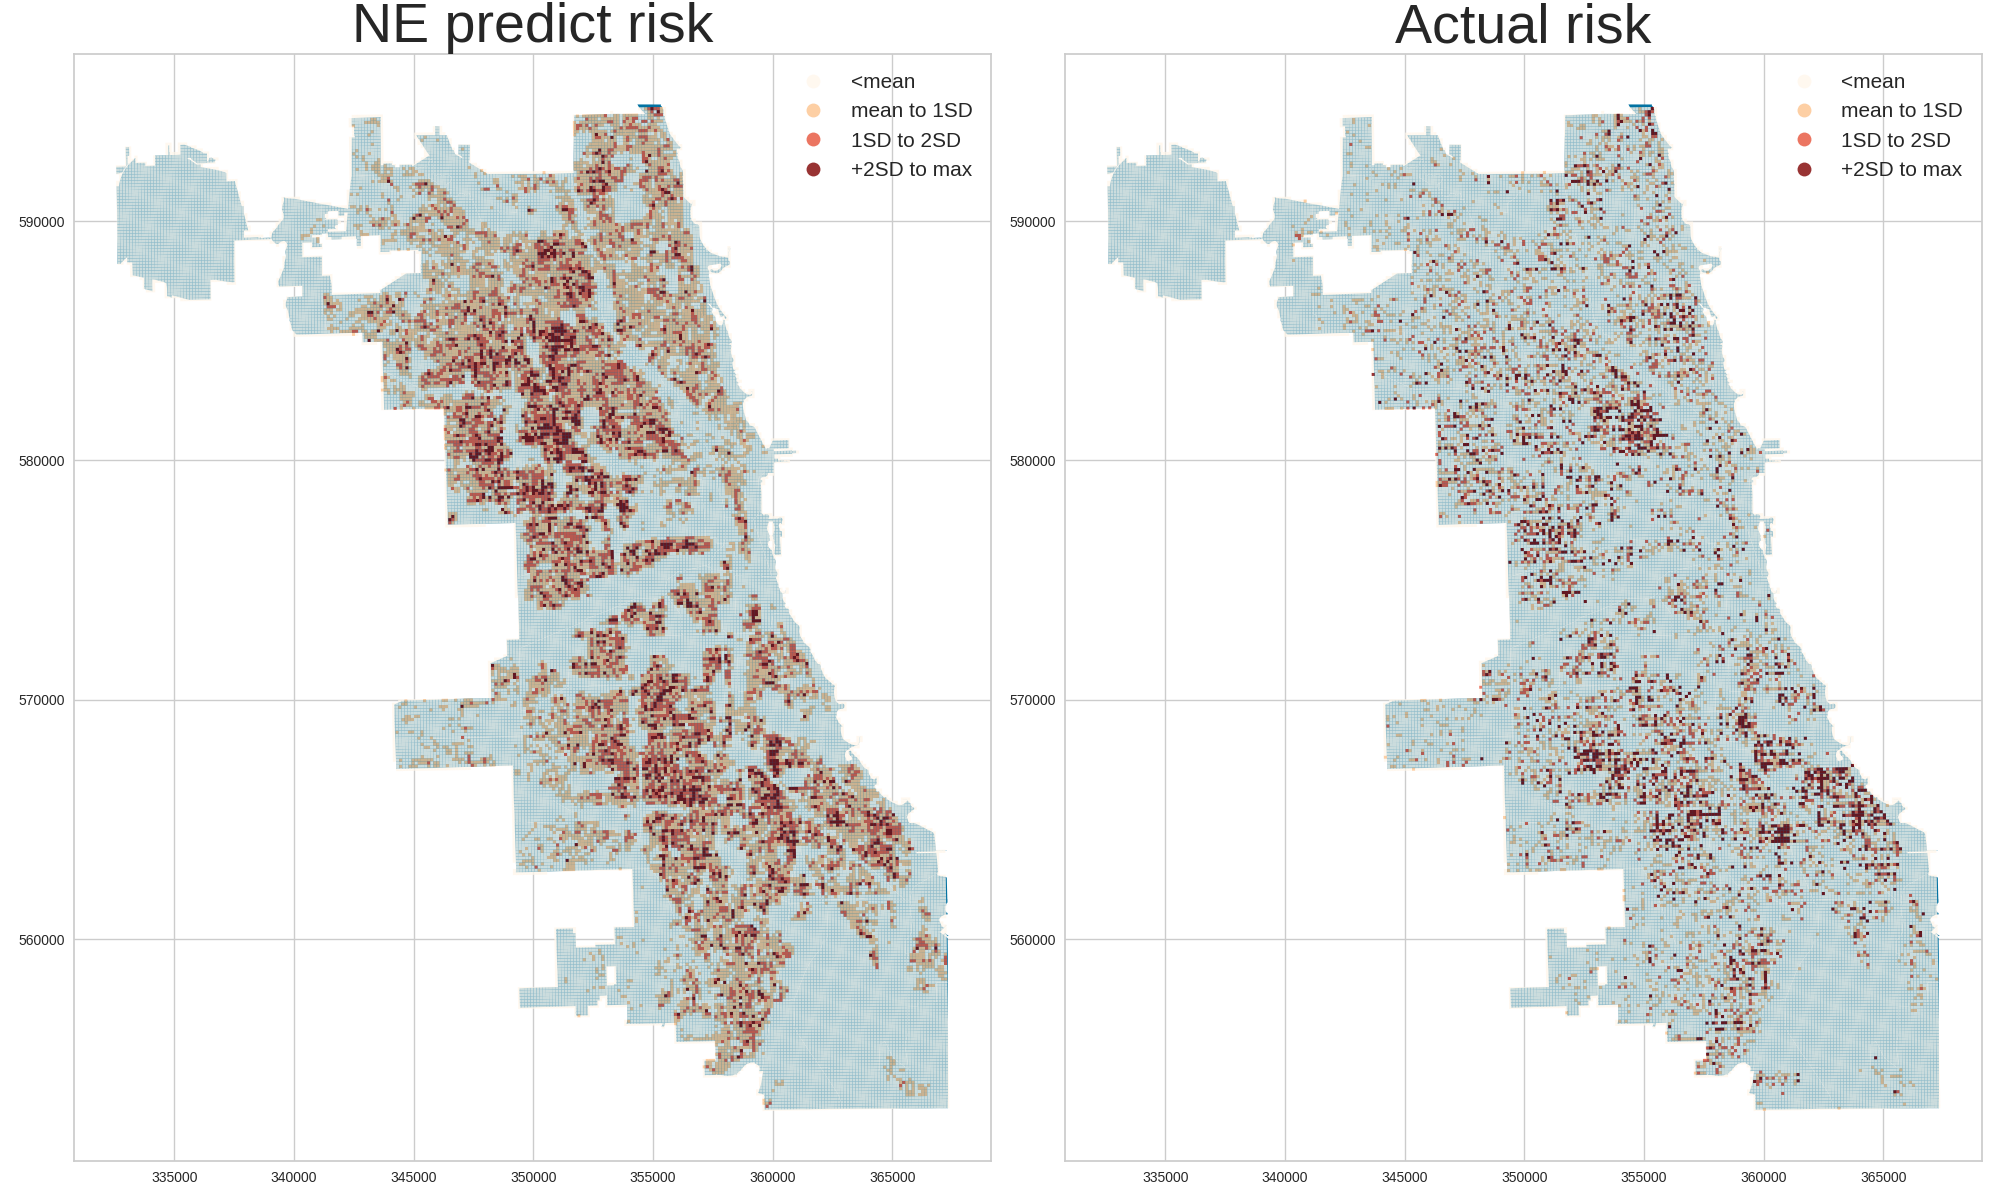
\includegraphics[scale=0.25]{./non-crime-timeseries-fig/NE_riskmap.png}
%   \caption{左:NEによるリスクマップ 右:実際のリスクマップ}
%   \label{fig:non-crime-timeseries-ne-risk}
% \end{figure}

% \begin{figure}
%   \centering % 図を中央寄せにする
%   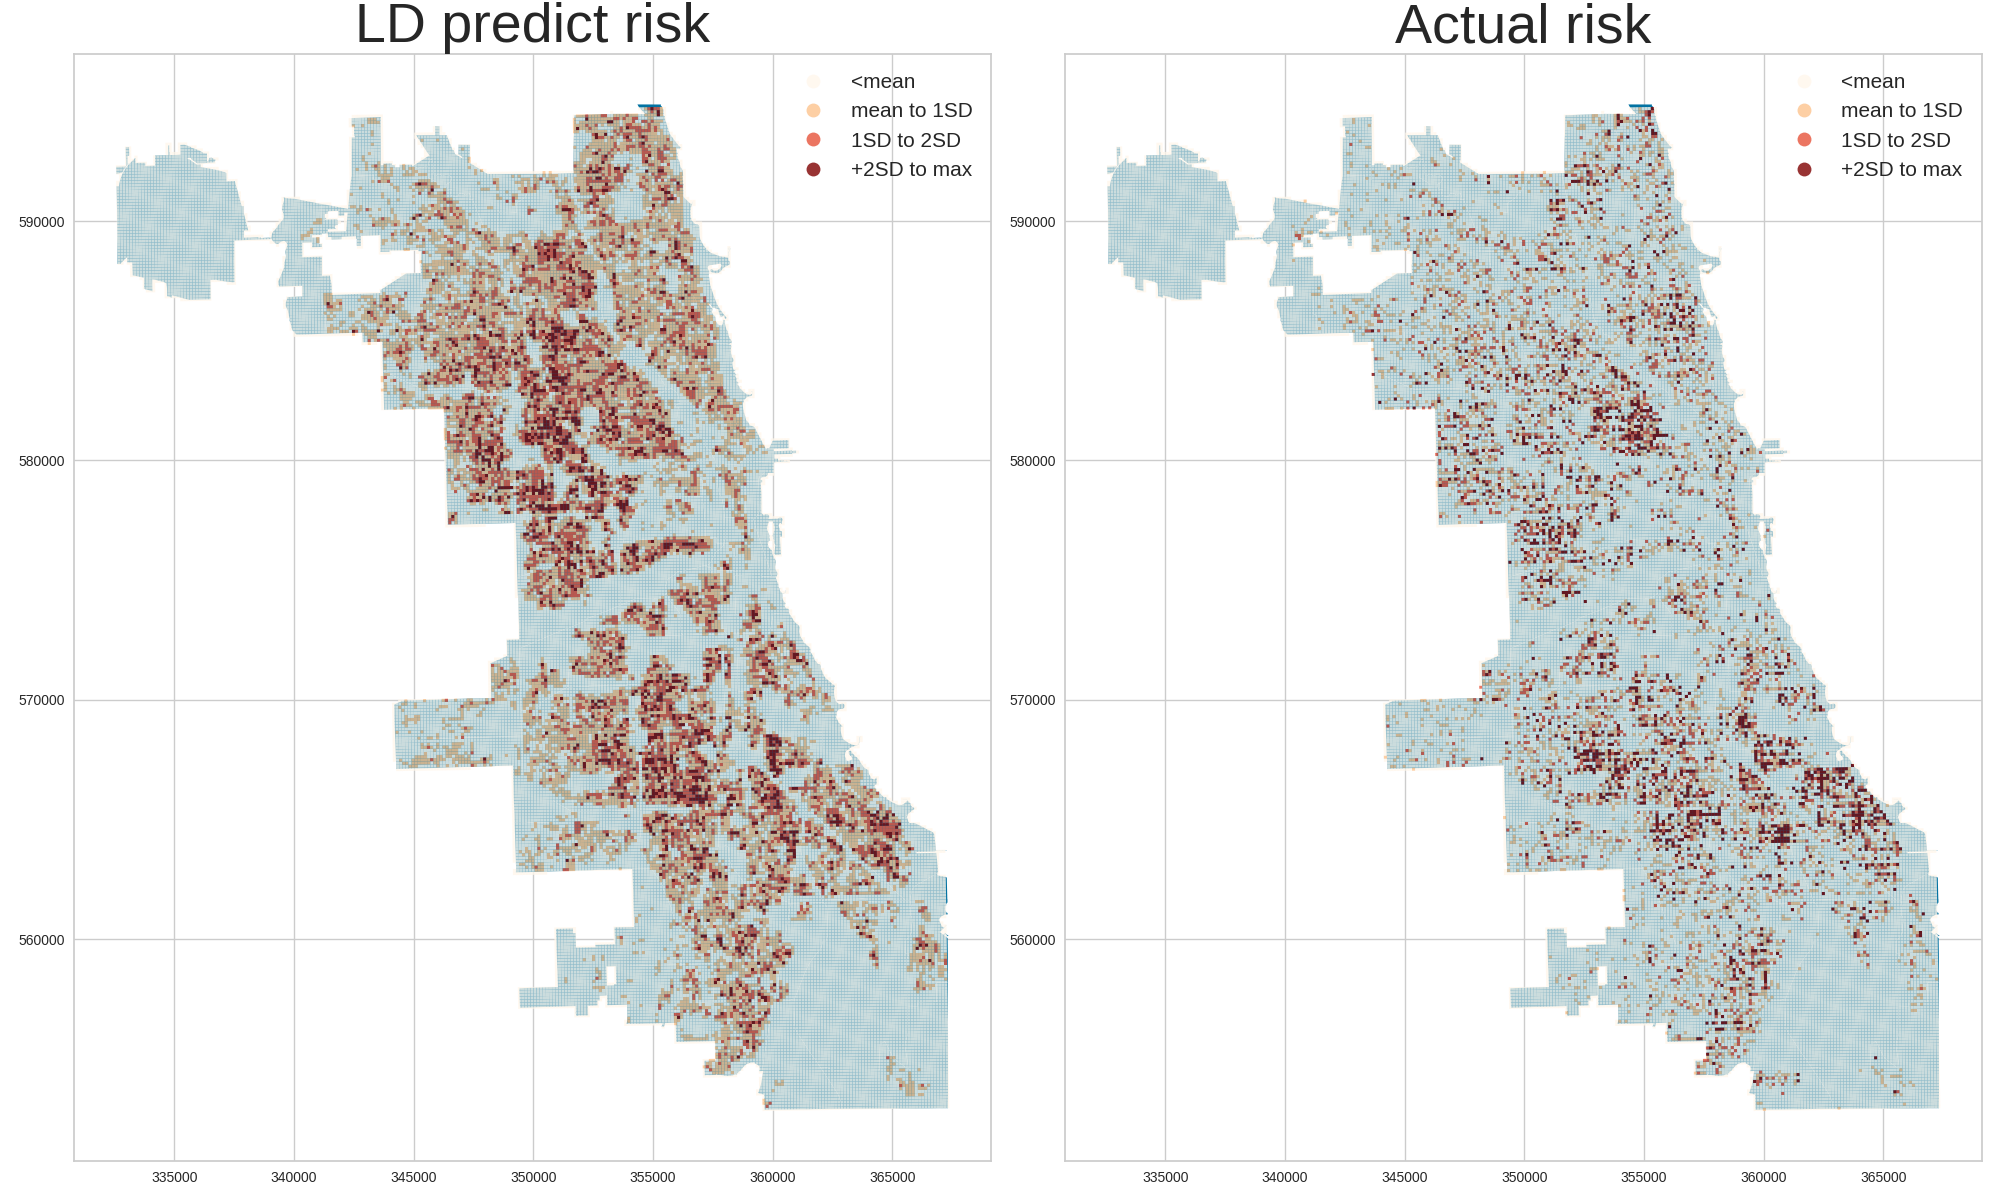
\includegraphics[scale=0.25]{./non-crime-timeseries-fig/LD_riskmap.png}
%   \caption{左:LDによるリスクマップ 右:実際のリスクマップ}
%   \label{fig:non-crime-timeseries-ld-risk}
% \end{figure}

% \begin{figure}
%   \centering % 図を中央寄せにする
%   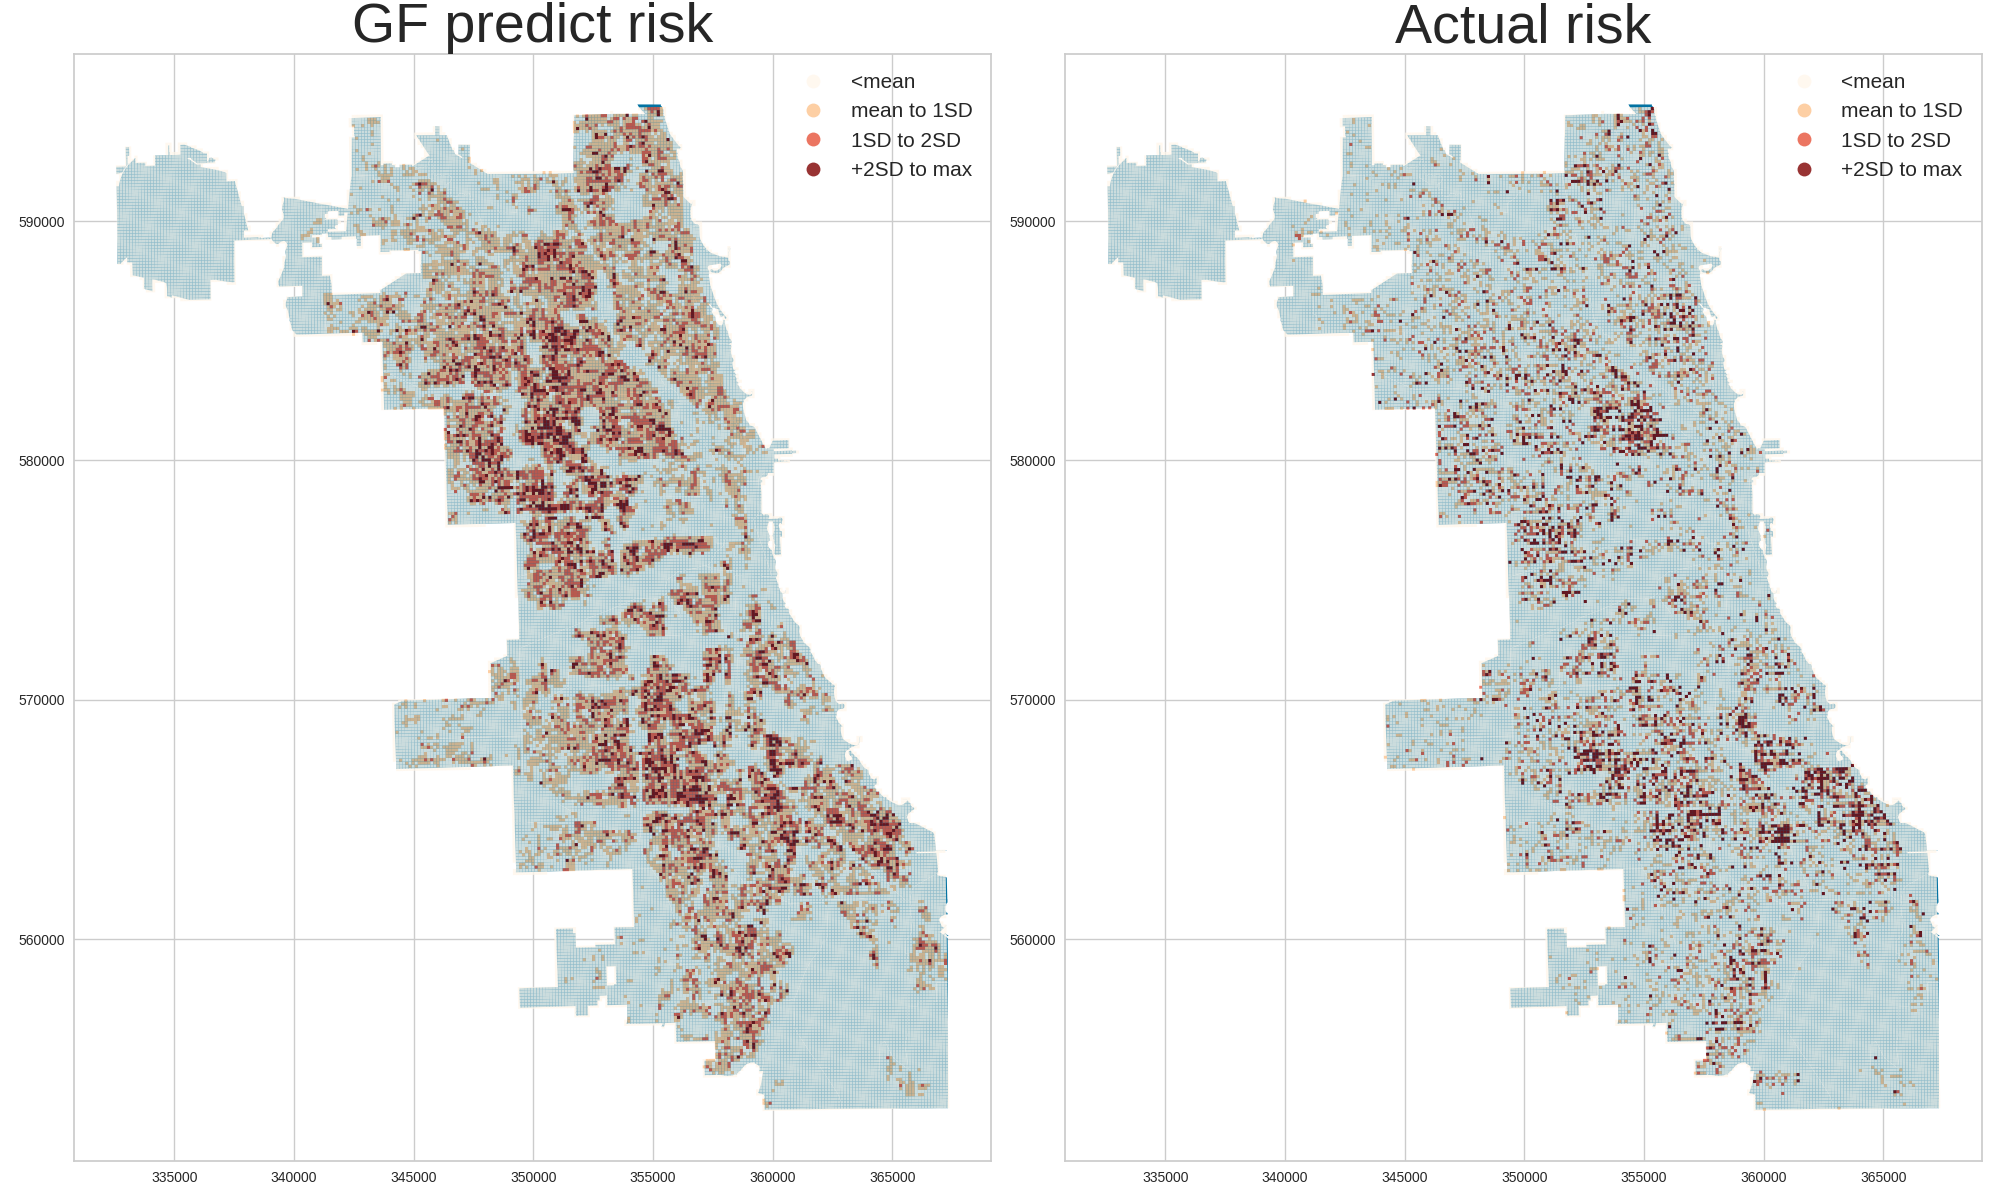
\includegraphics[scale=0.25]{./non-crime-timeseries-fig/GF_riskmap.png}
%   \caption{左:GFによるリスクマップ 右:実際のリスクマップ}
%   \label{fig:non-crime-timeseries-gf-risk}
% \end{figure}

% \begin{figure}
%   \centering % 図を中央寄せにする
%   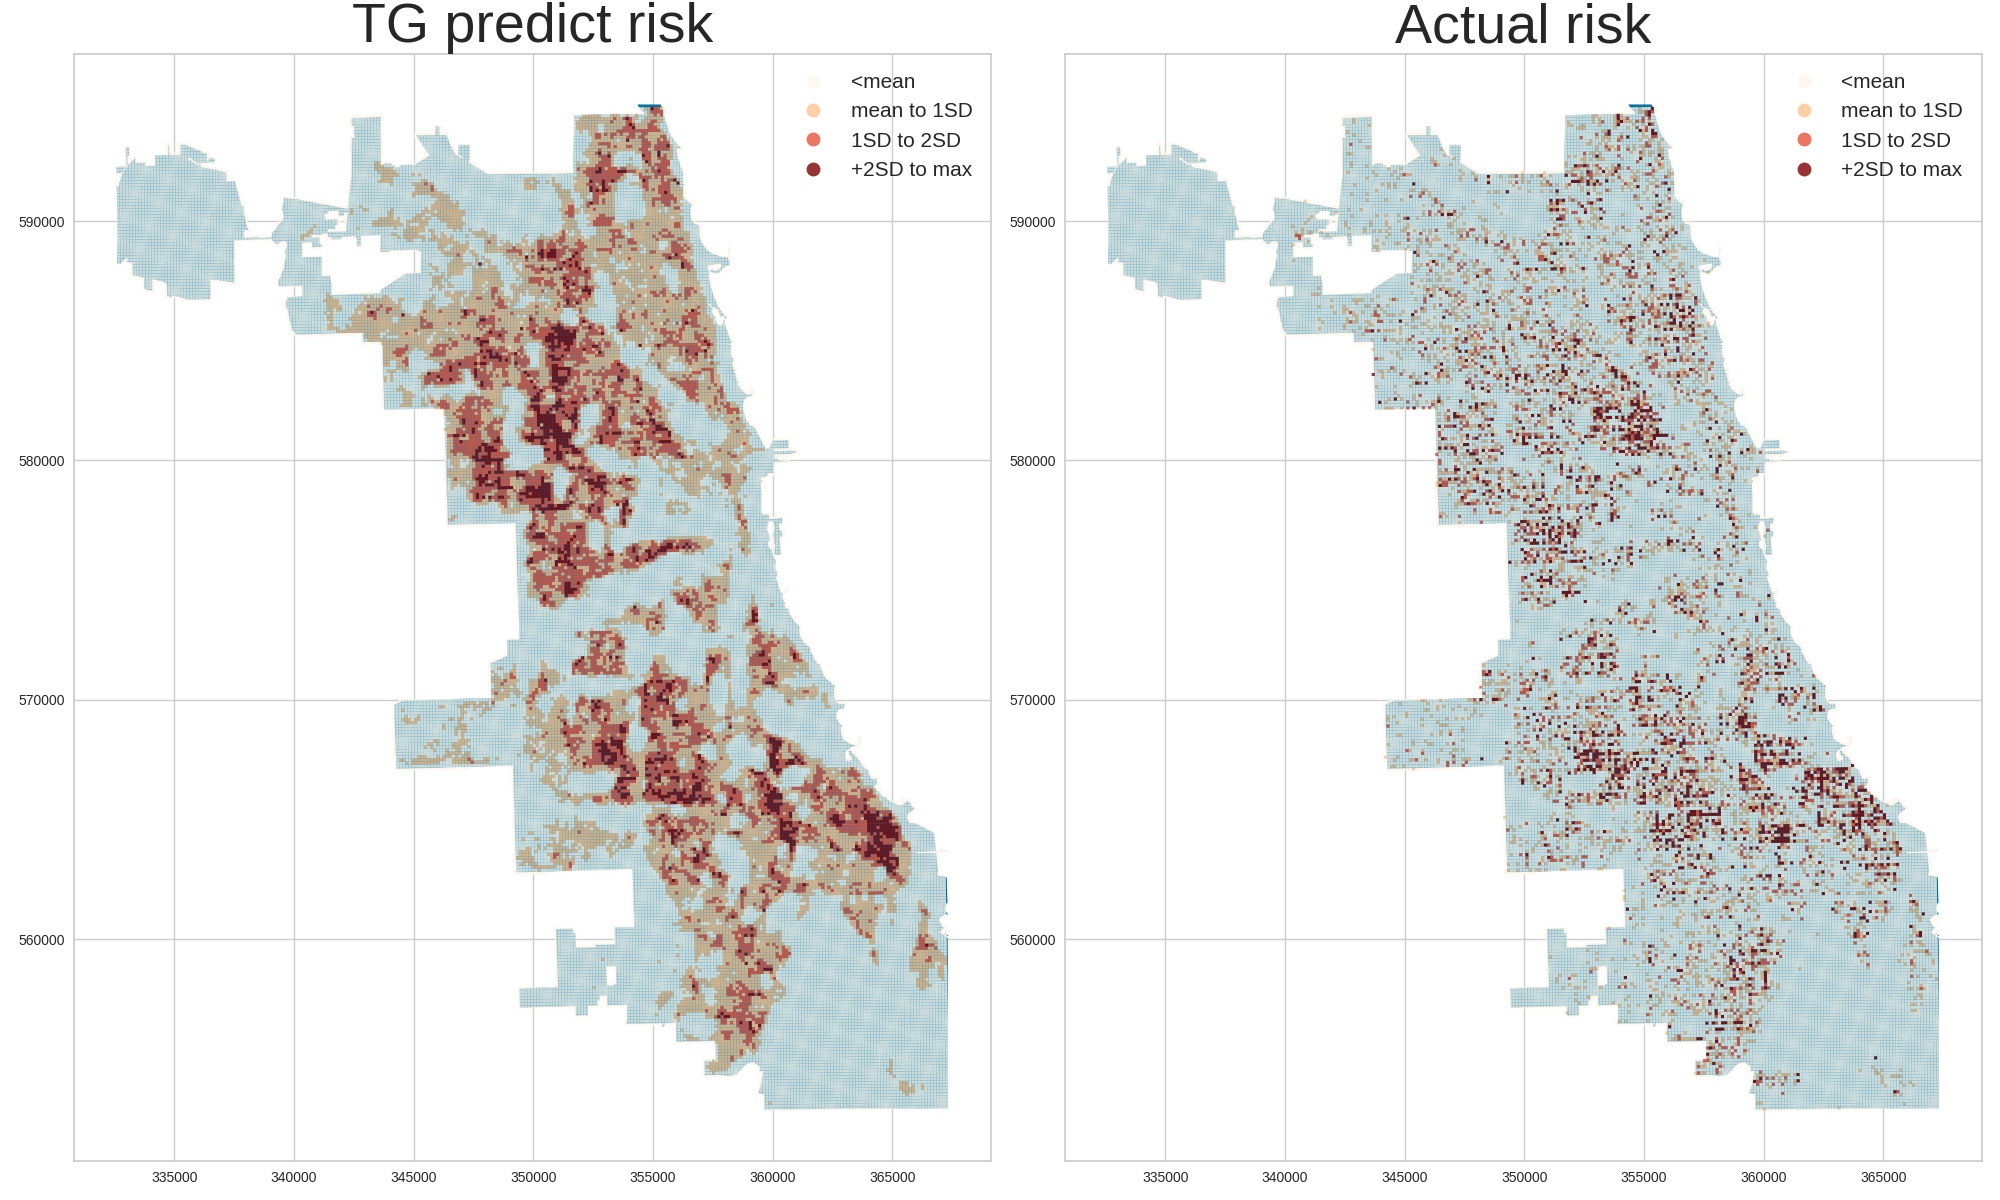
\includegraphics[scale=0.25]{./non-crime-timeseries-fig/TG_riskmap.png}
%   \caption{左:TGによるリスクマップ 右:実際のリスクマップ}
%   \label{fig:non-crime-timeseries-tg-risk}
% \end{figure}

% \begin{figure}
%   \centering % 図を中央寄せにする
%   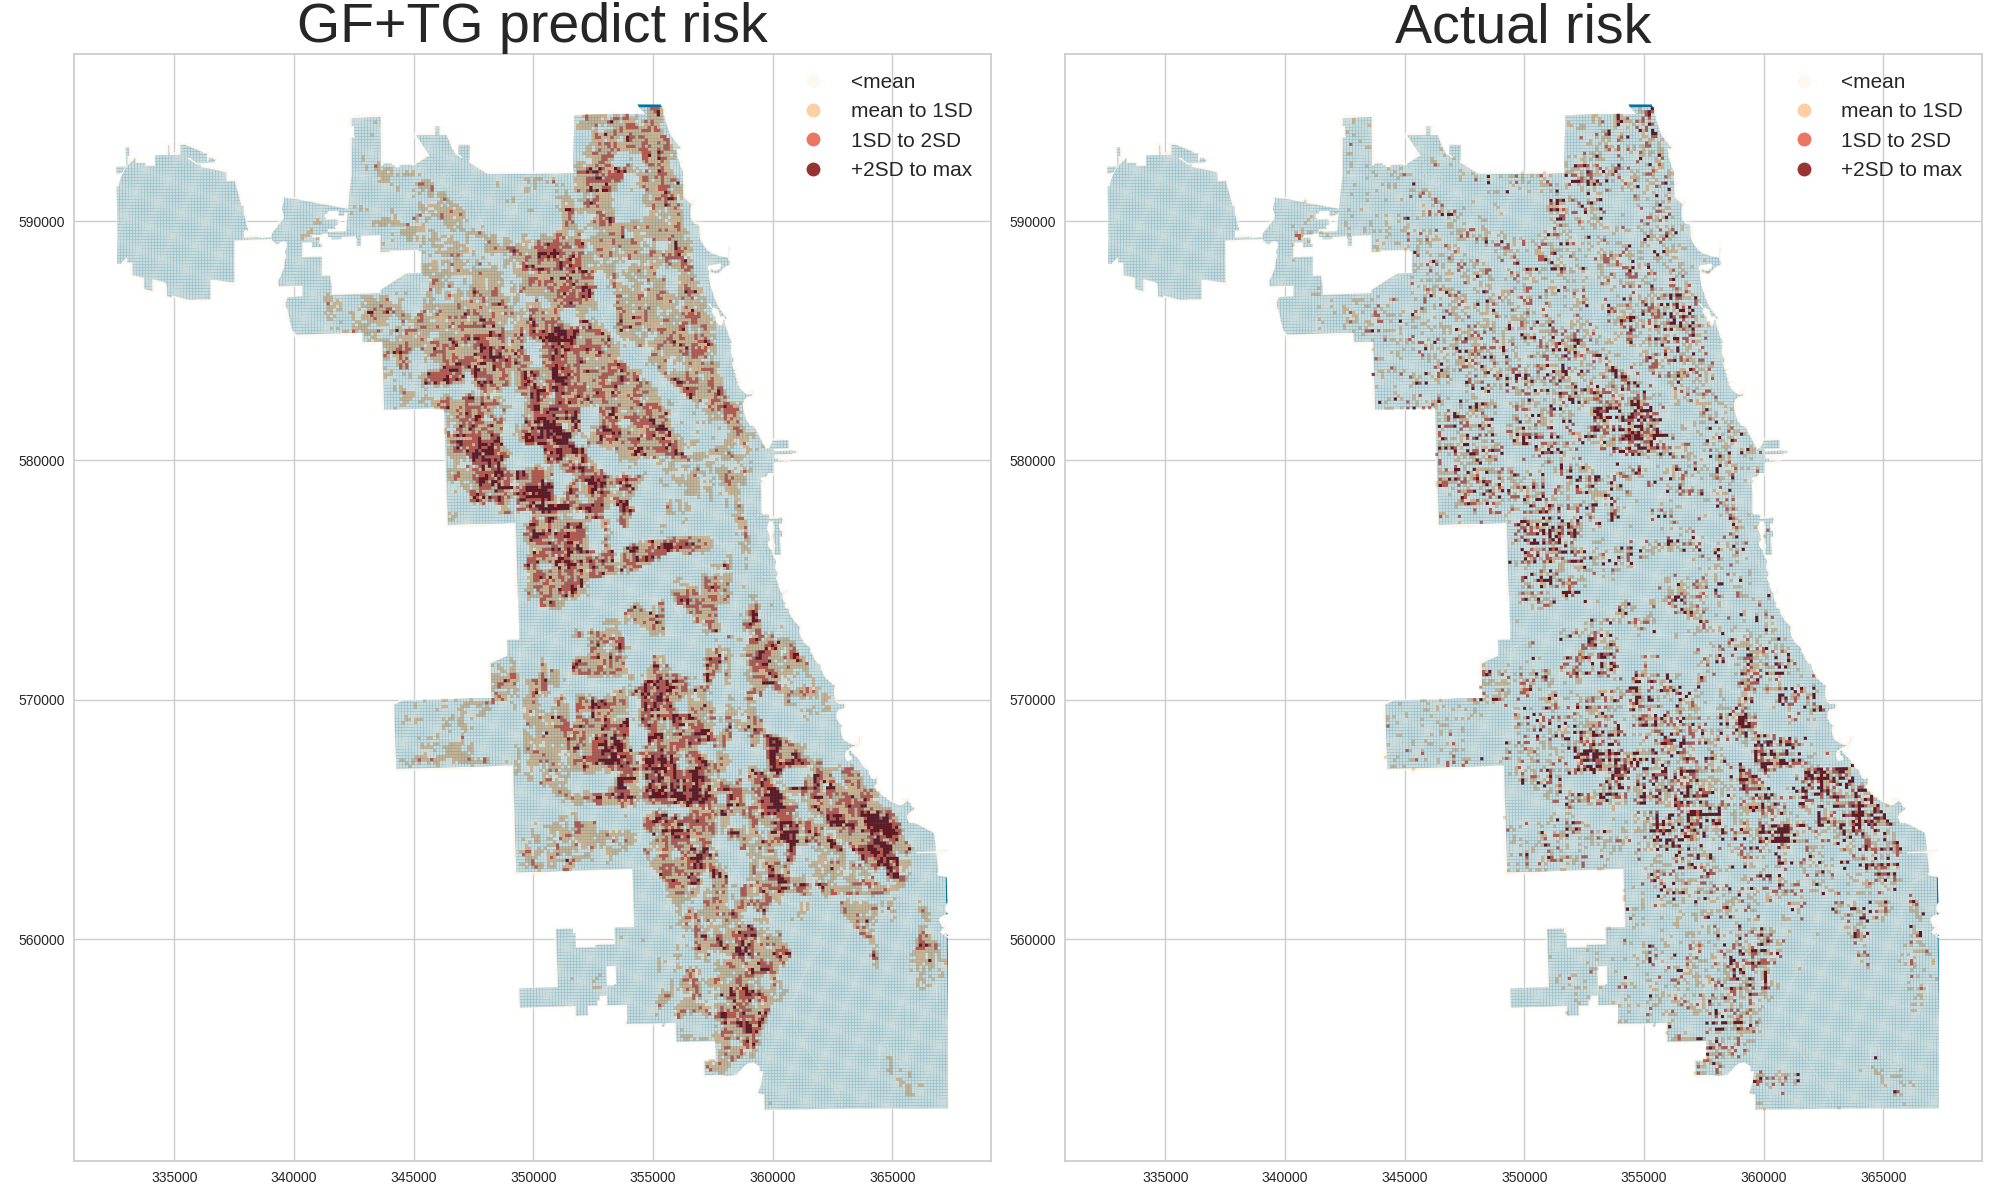
\includegraphics[scale=0.25]{./non-crime-timeseries-fig/GF+TG_riskmap.png}
%   \caption{左:FG+TGによるリスクマップ 右:実際のリスクマップ}
%   \label{fig:non-crime-timeseries-gf-tg-risk}
% \end{figure}
% %------------------------------------------
% % confusion matrix
% %------------------------------------------
% \begin{figure}
%   \centering % 図を中央寄せにする
%   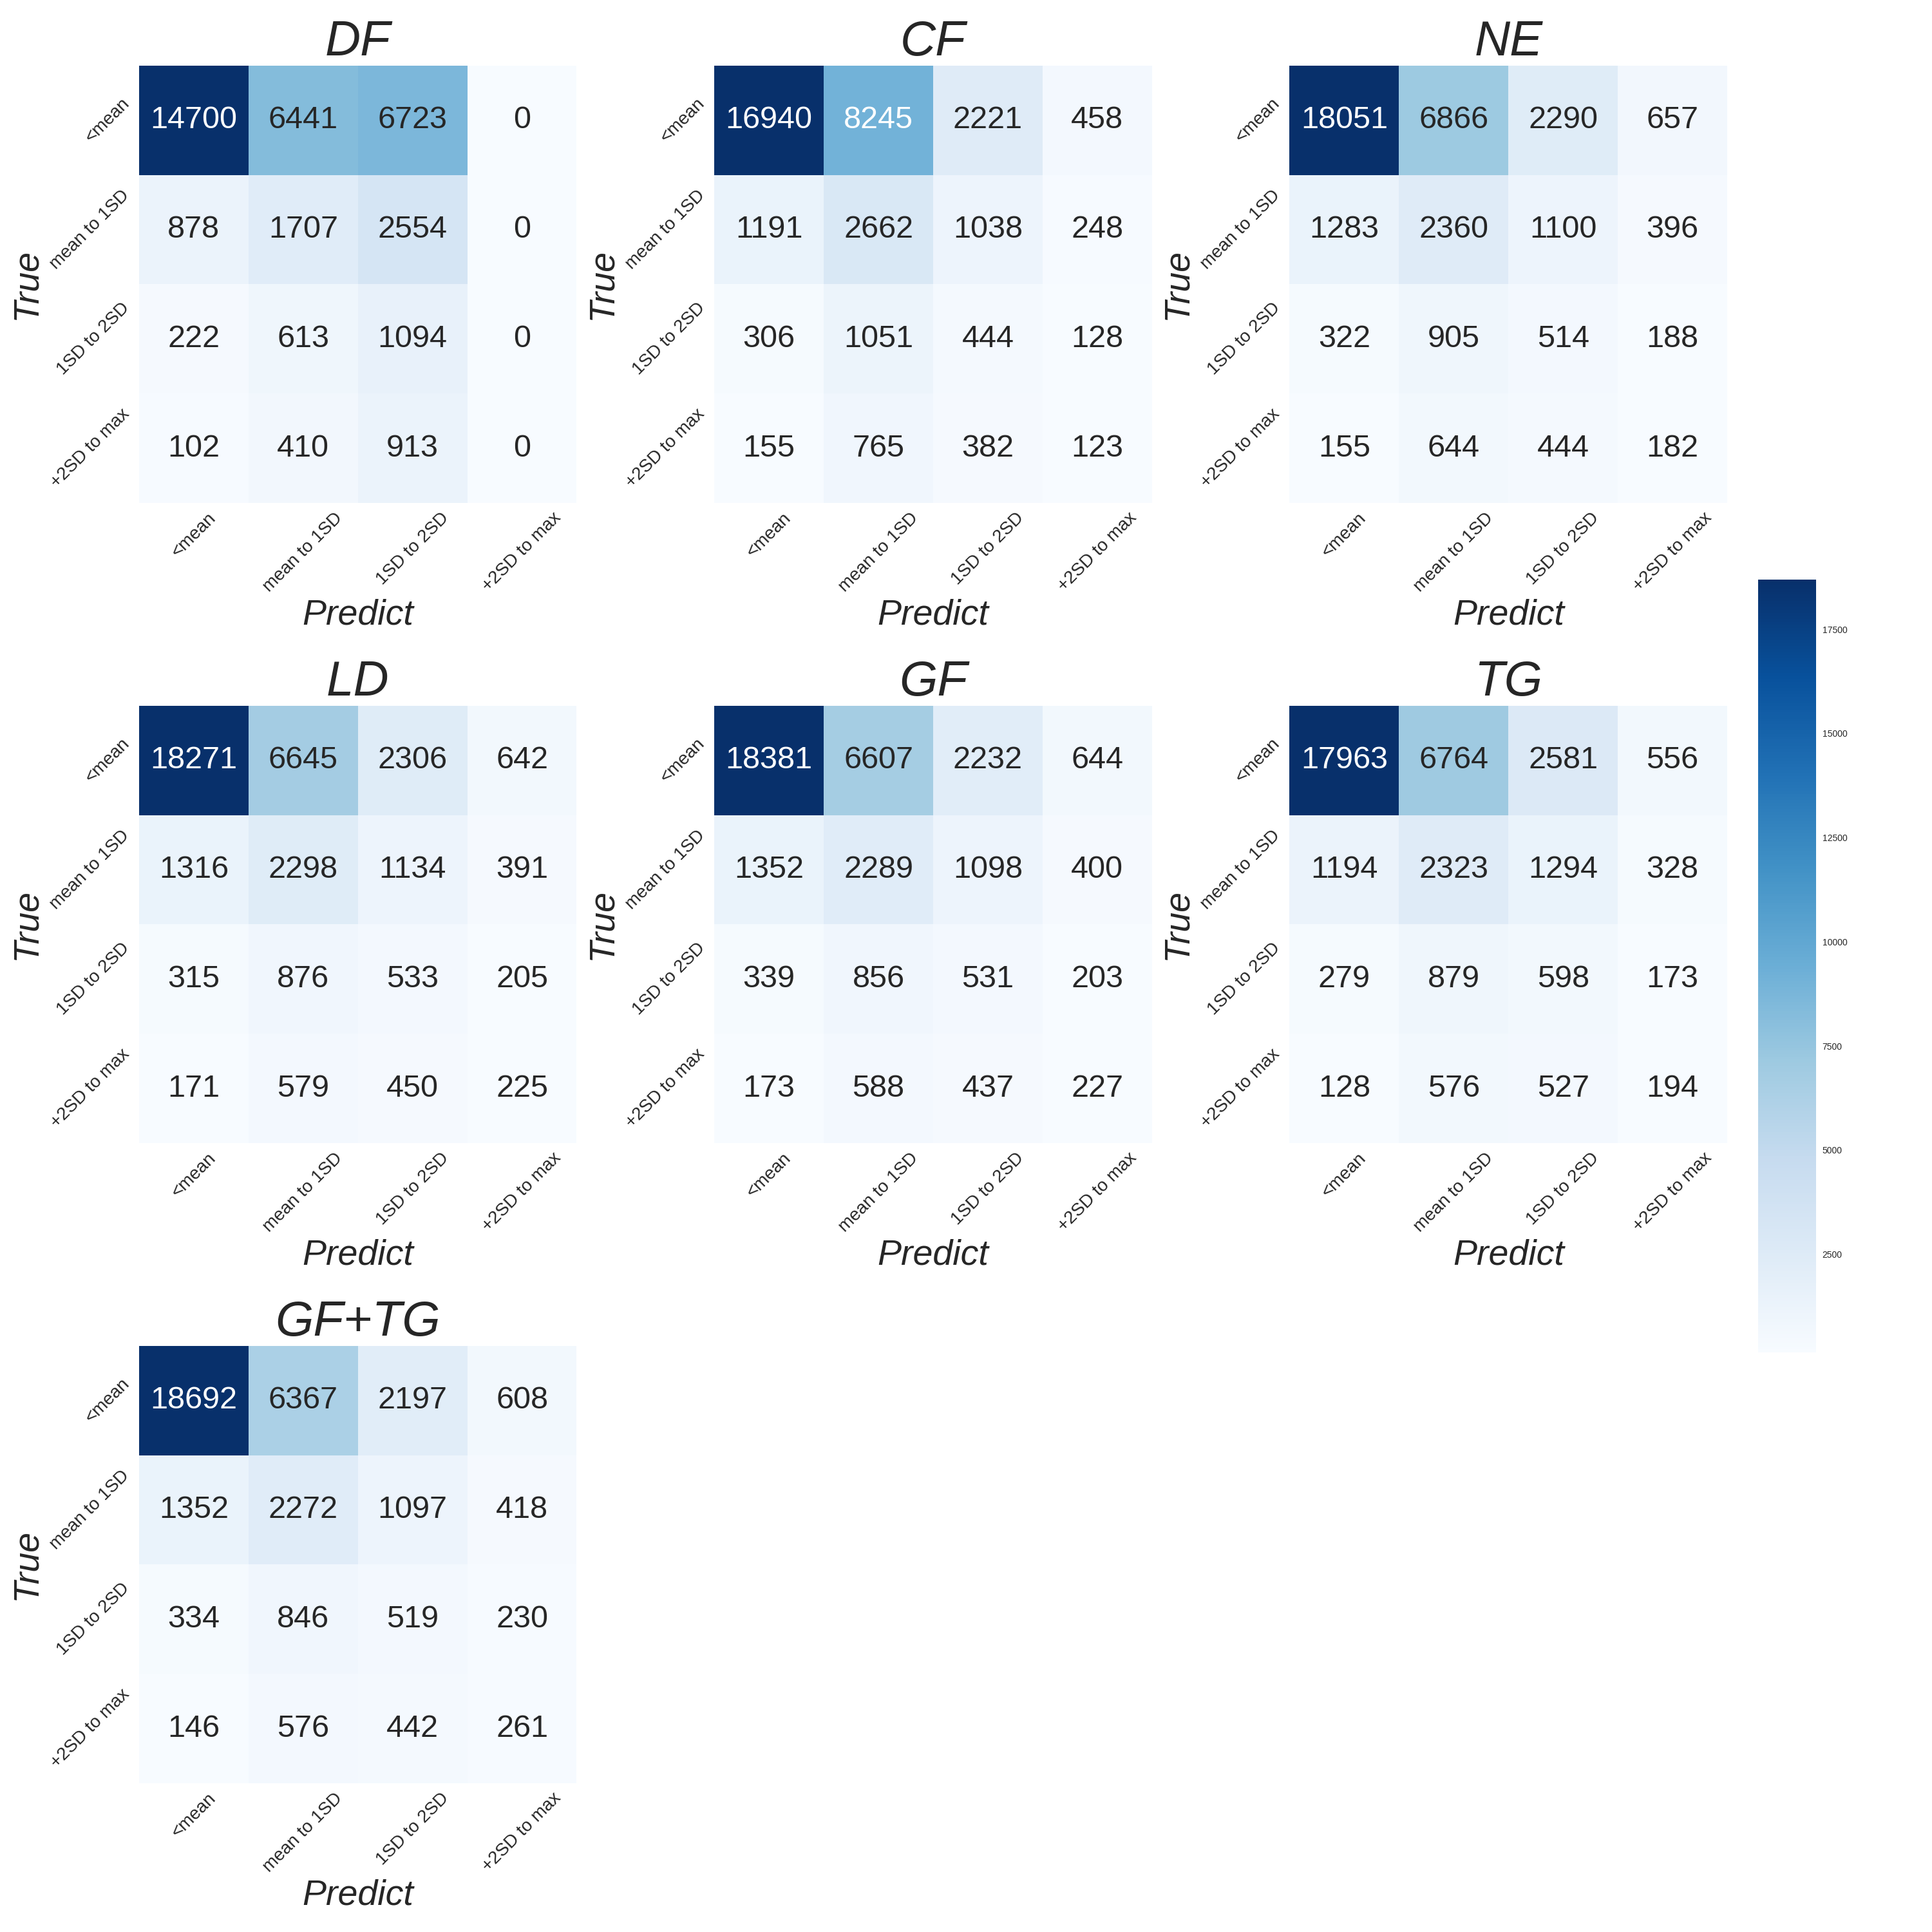
\includegraphics[scale=0.16]{./non-crime-timeseries-fig/non_crime_timeseries_four_cm.png}
%   \caption{4カテゴリーの混同行列}
%   \label{fig:non-crime-timeseries-4cm}
% \end{figure}

% \begin{figure}
%   \centering % 図を中央寄せにする
%   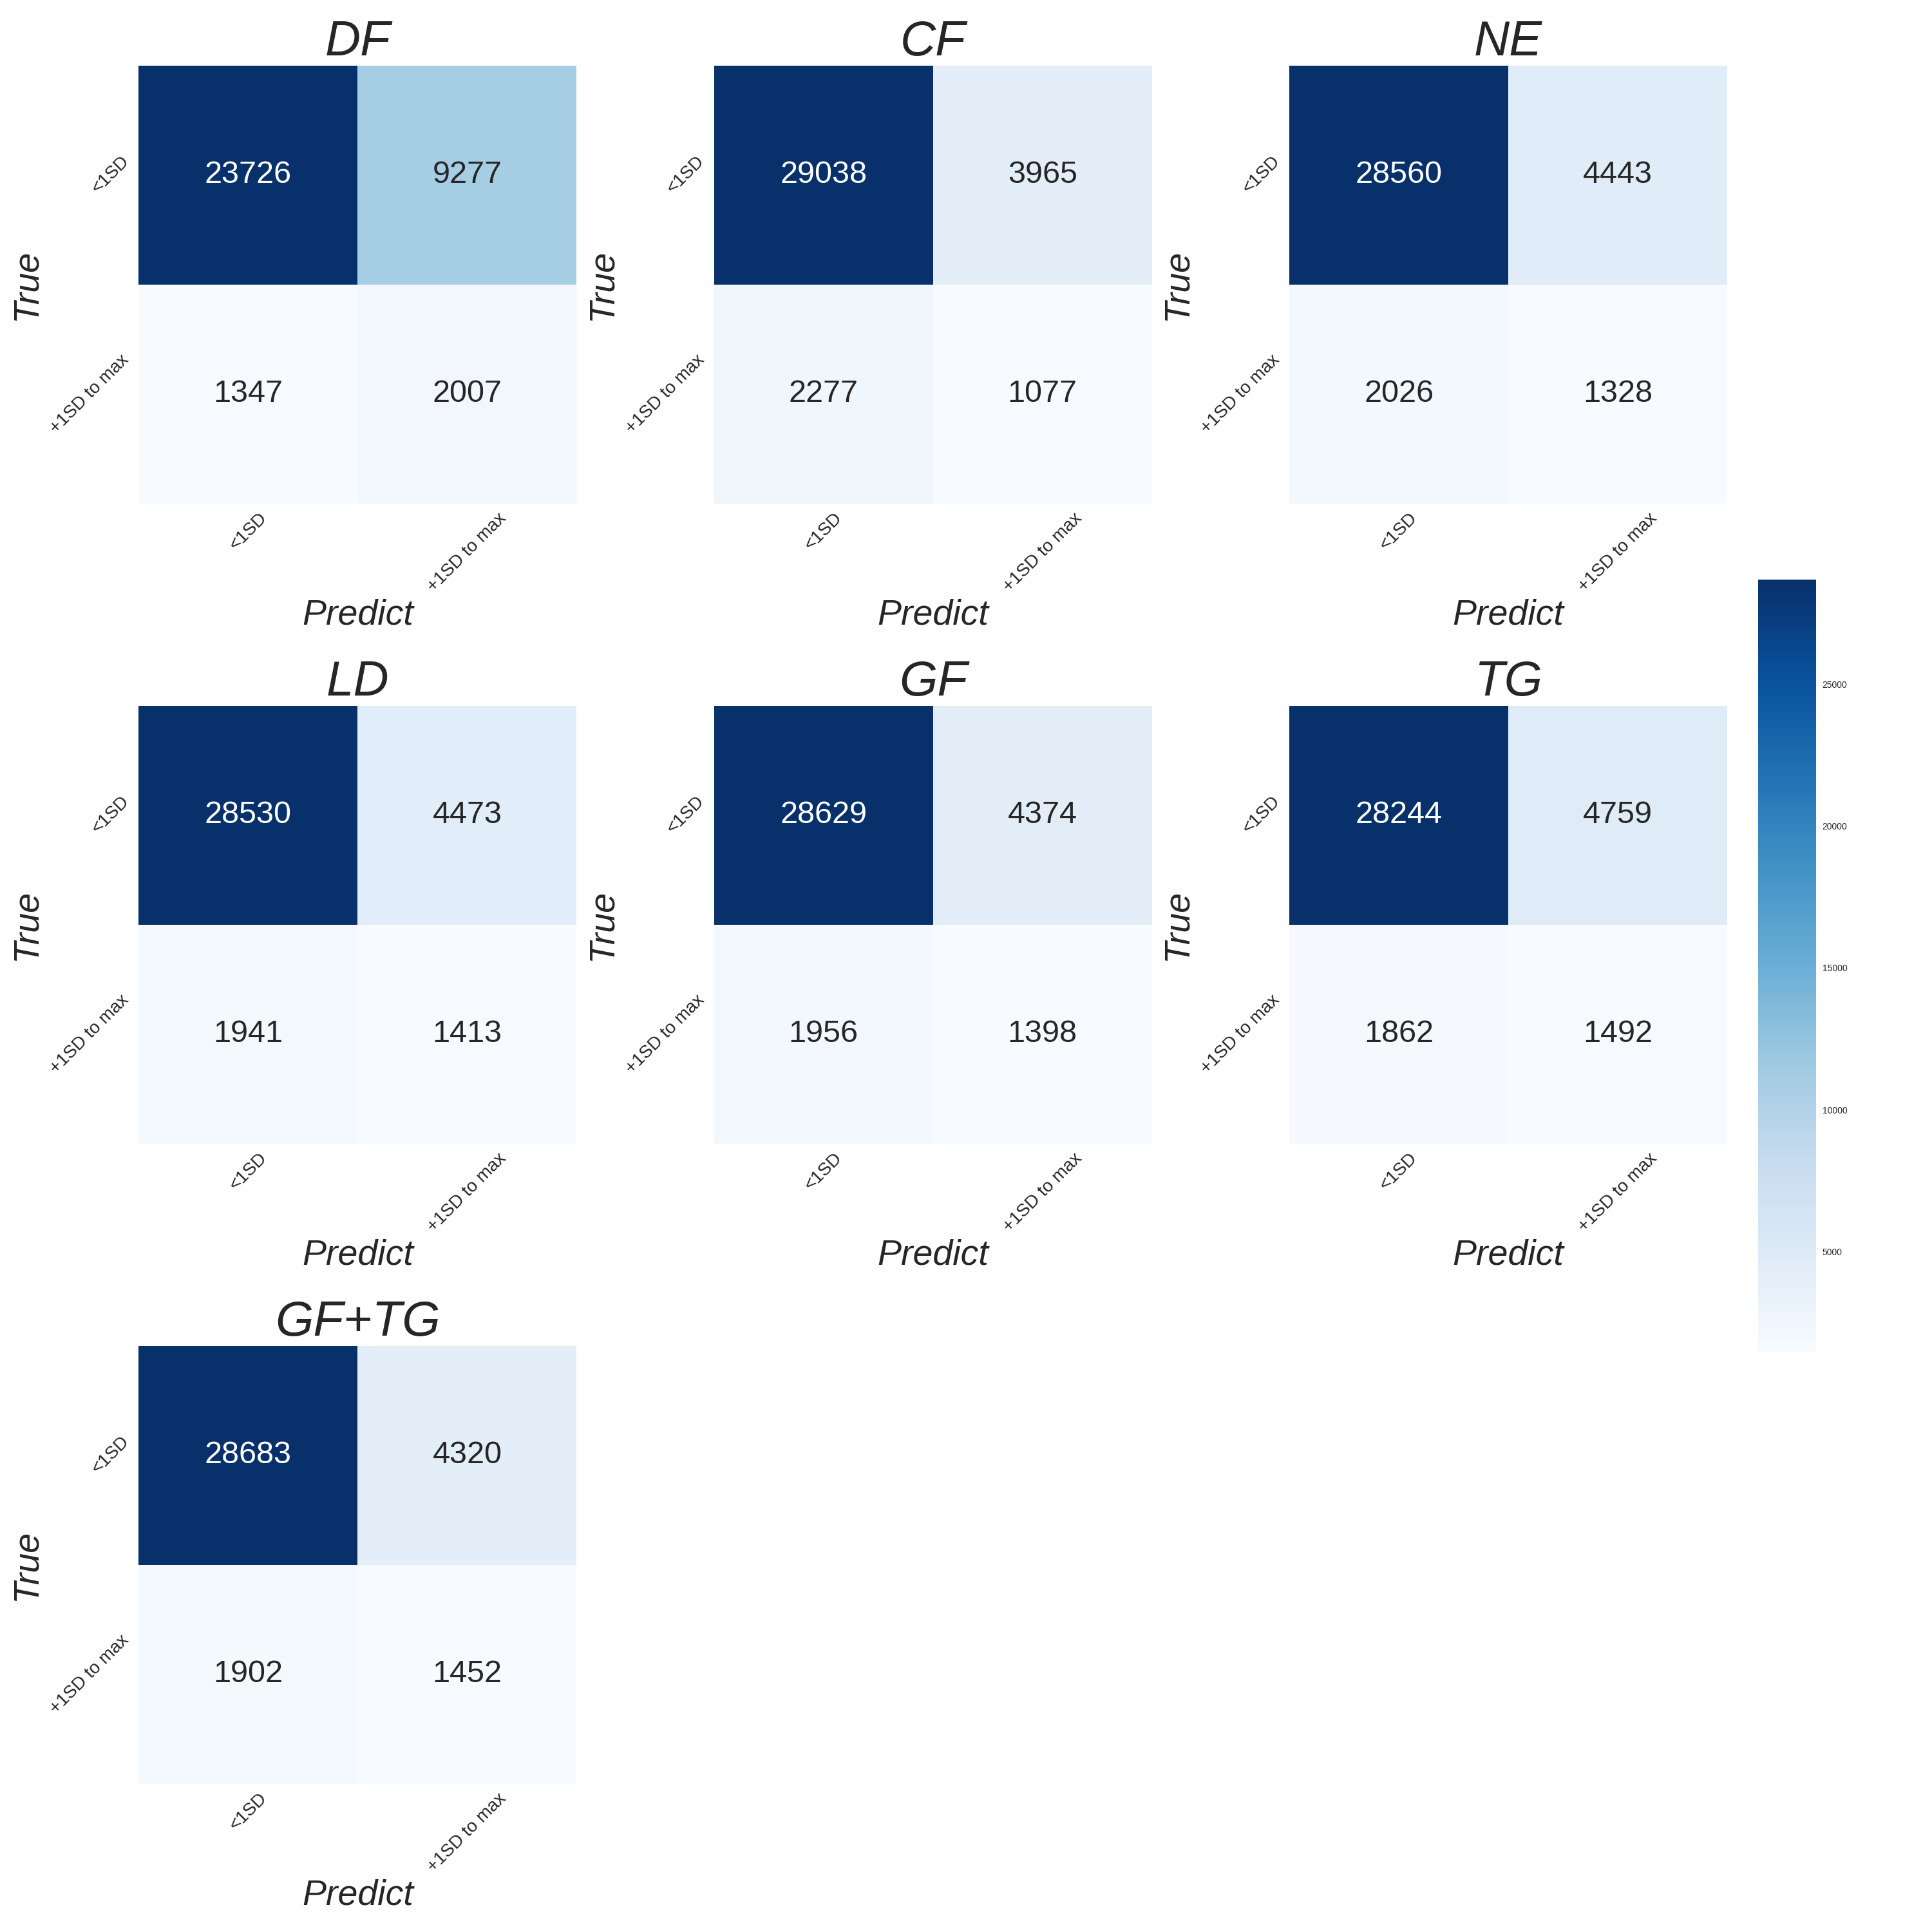
\includegraphics[scale=0.16]{./non-crime-timeseries-fig/non_crime_timeseries_two_cm.png}
%   \caption{2カテゴリーの混同行列}
%   \label{fig:non-crime-timeseries-2cm}
% \end{figure}
% ---------------------------------
% FNFPplot
% ---------------------------------
% \begin{figure}
%   \centering % 図を中央寄せにする
%   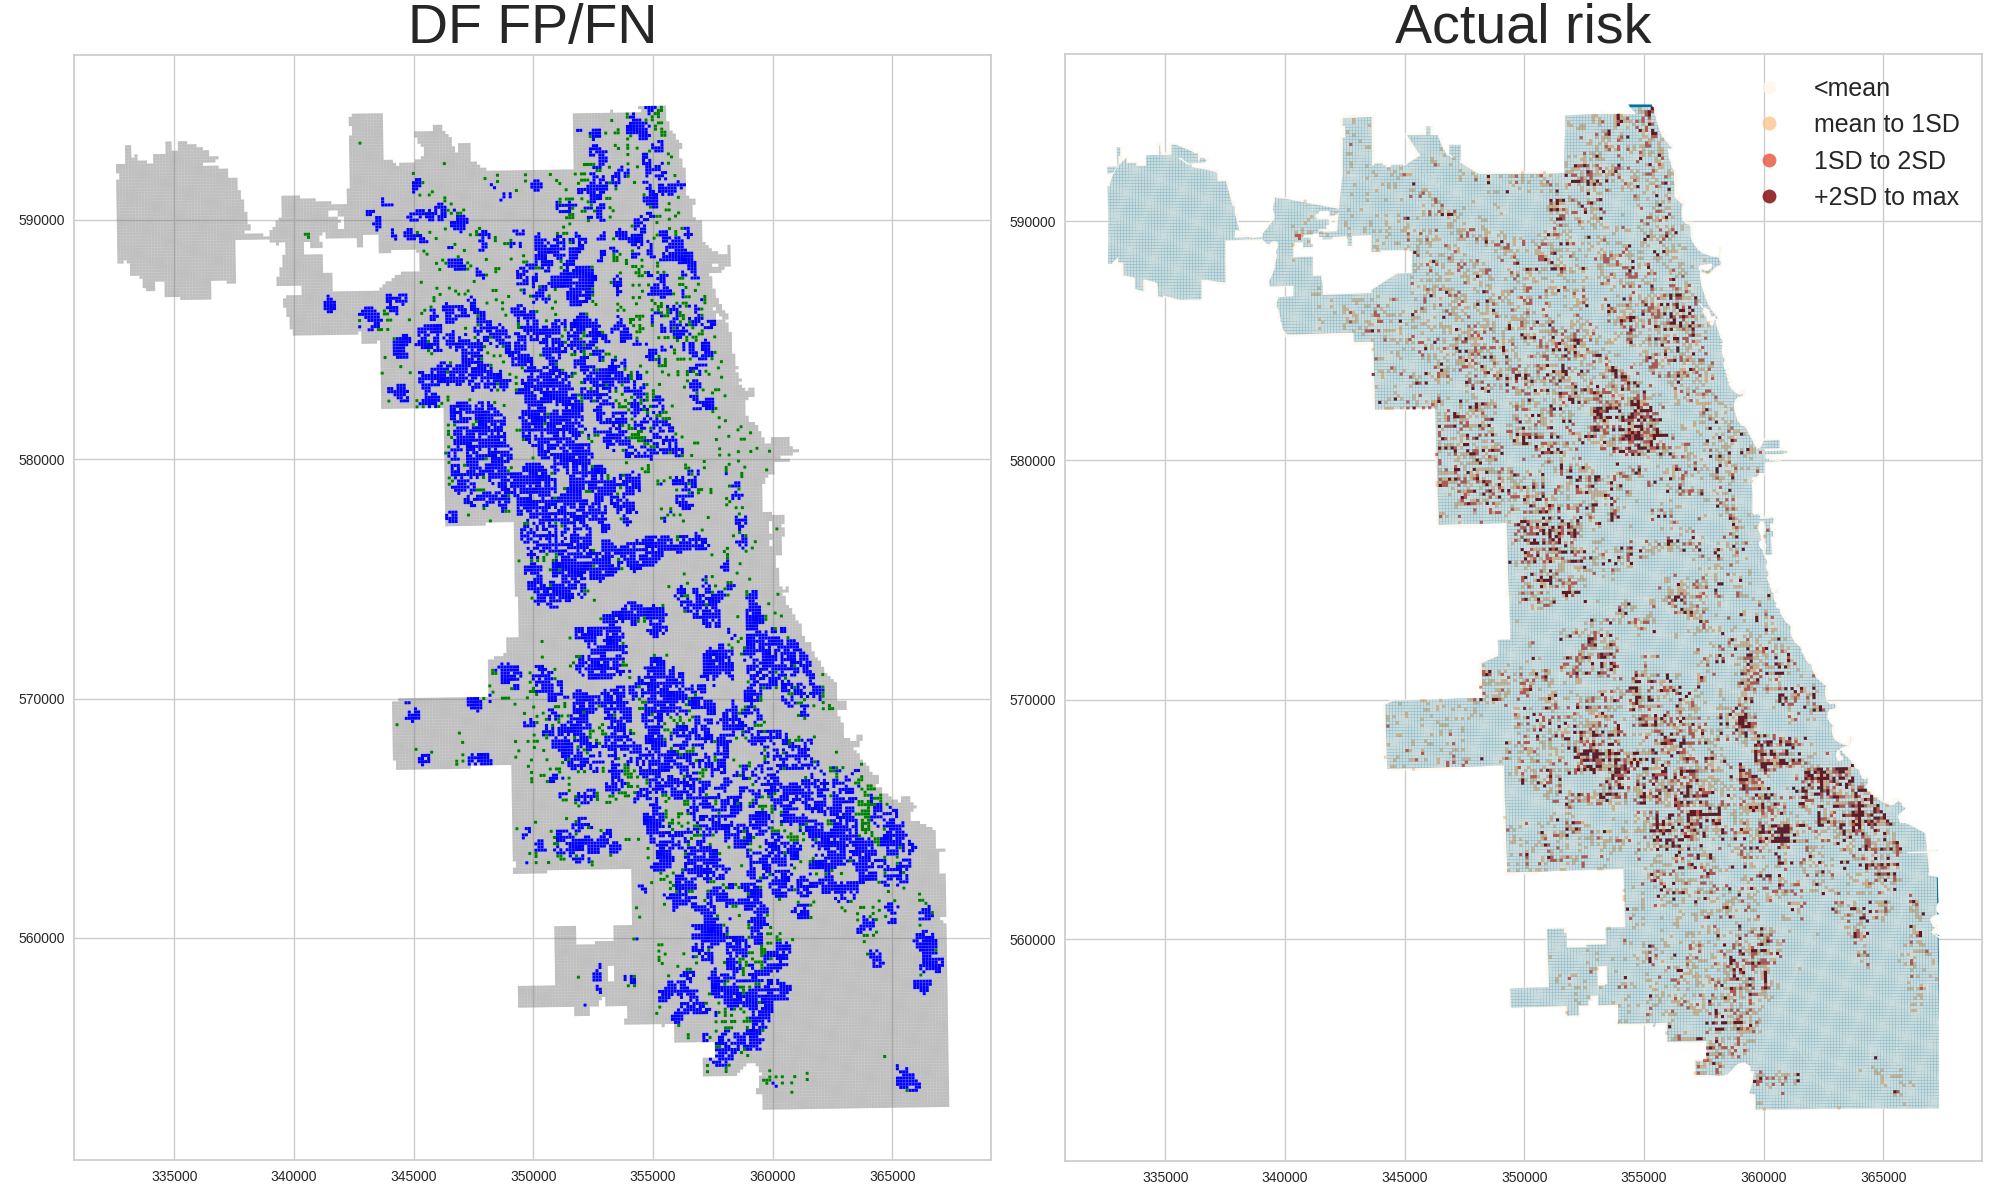
\includegraphics[scale=0.25]{./non-crime-timeseries-fig/DF_fnp.png}
%   \caption{左:DFのFPFN 右:実際のリスクマップ}
%   \label{fig:non-crime-timeseries-df-fnp}
% \end{figure}

% \begin{figure}
%   \centering % 図を中央寄せにする
%   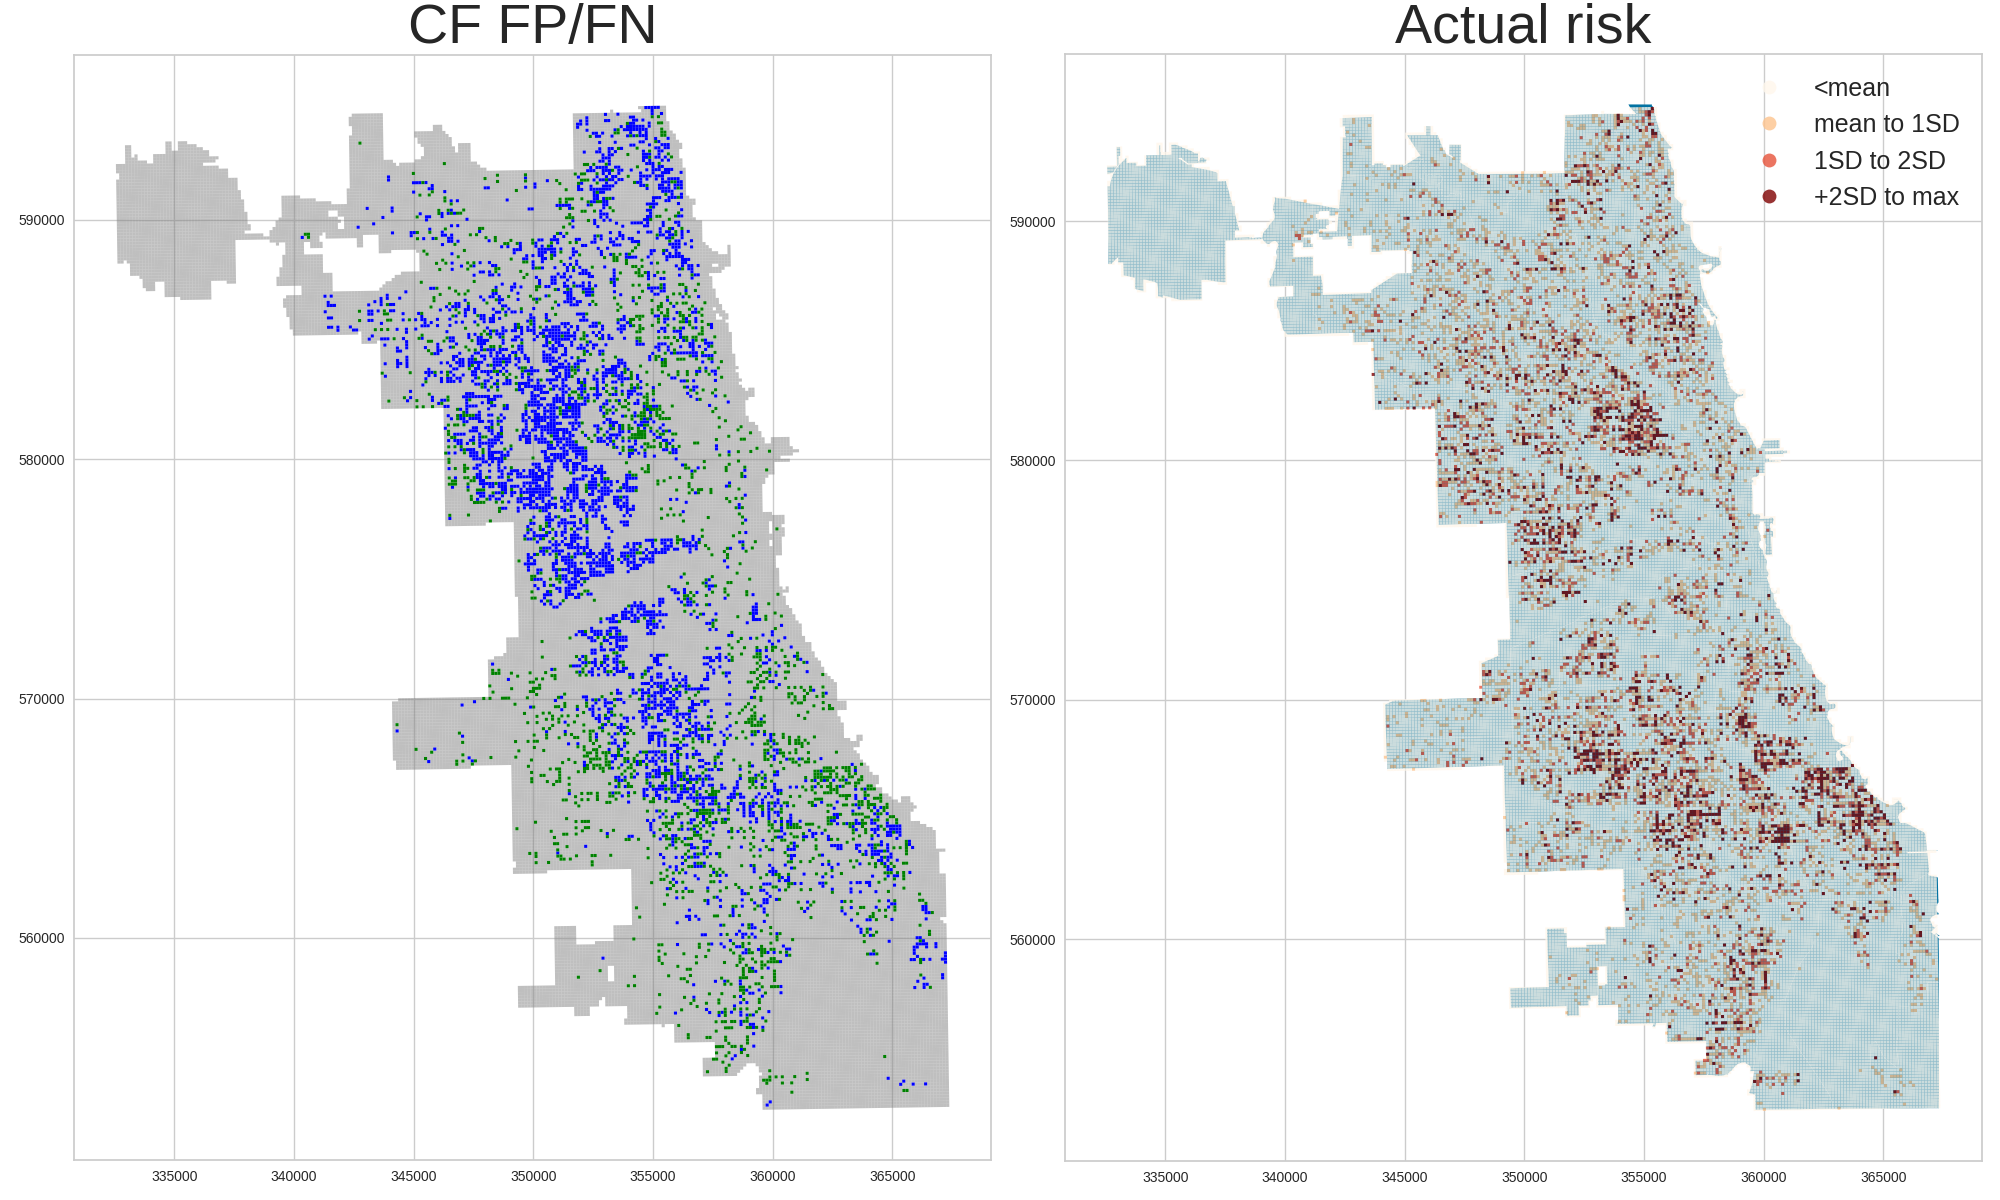
\includegraphics[scale=0.25]{./non-crime-timeseries-fig/CF_fnp.png}
%   \caption{左:CFのFPFN 右:実際のリスクマップ}
%   \label{fig:non-crime-timeseries-cf-fnp}
% \end{figure}

% \begin{figure}
%   \centering % 図を中央寄せにする
%   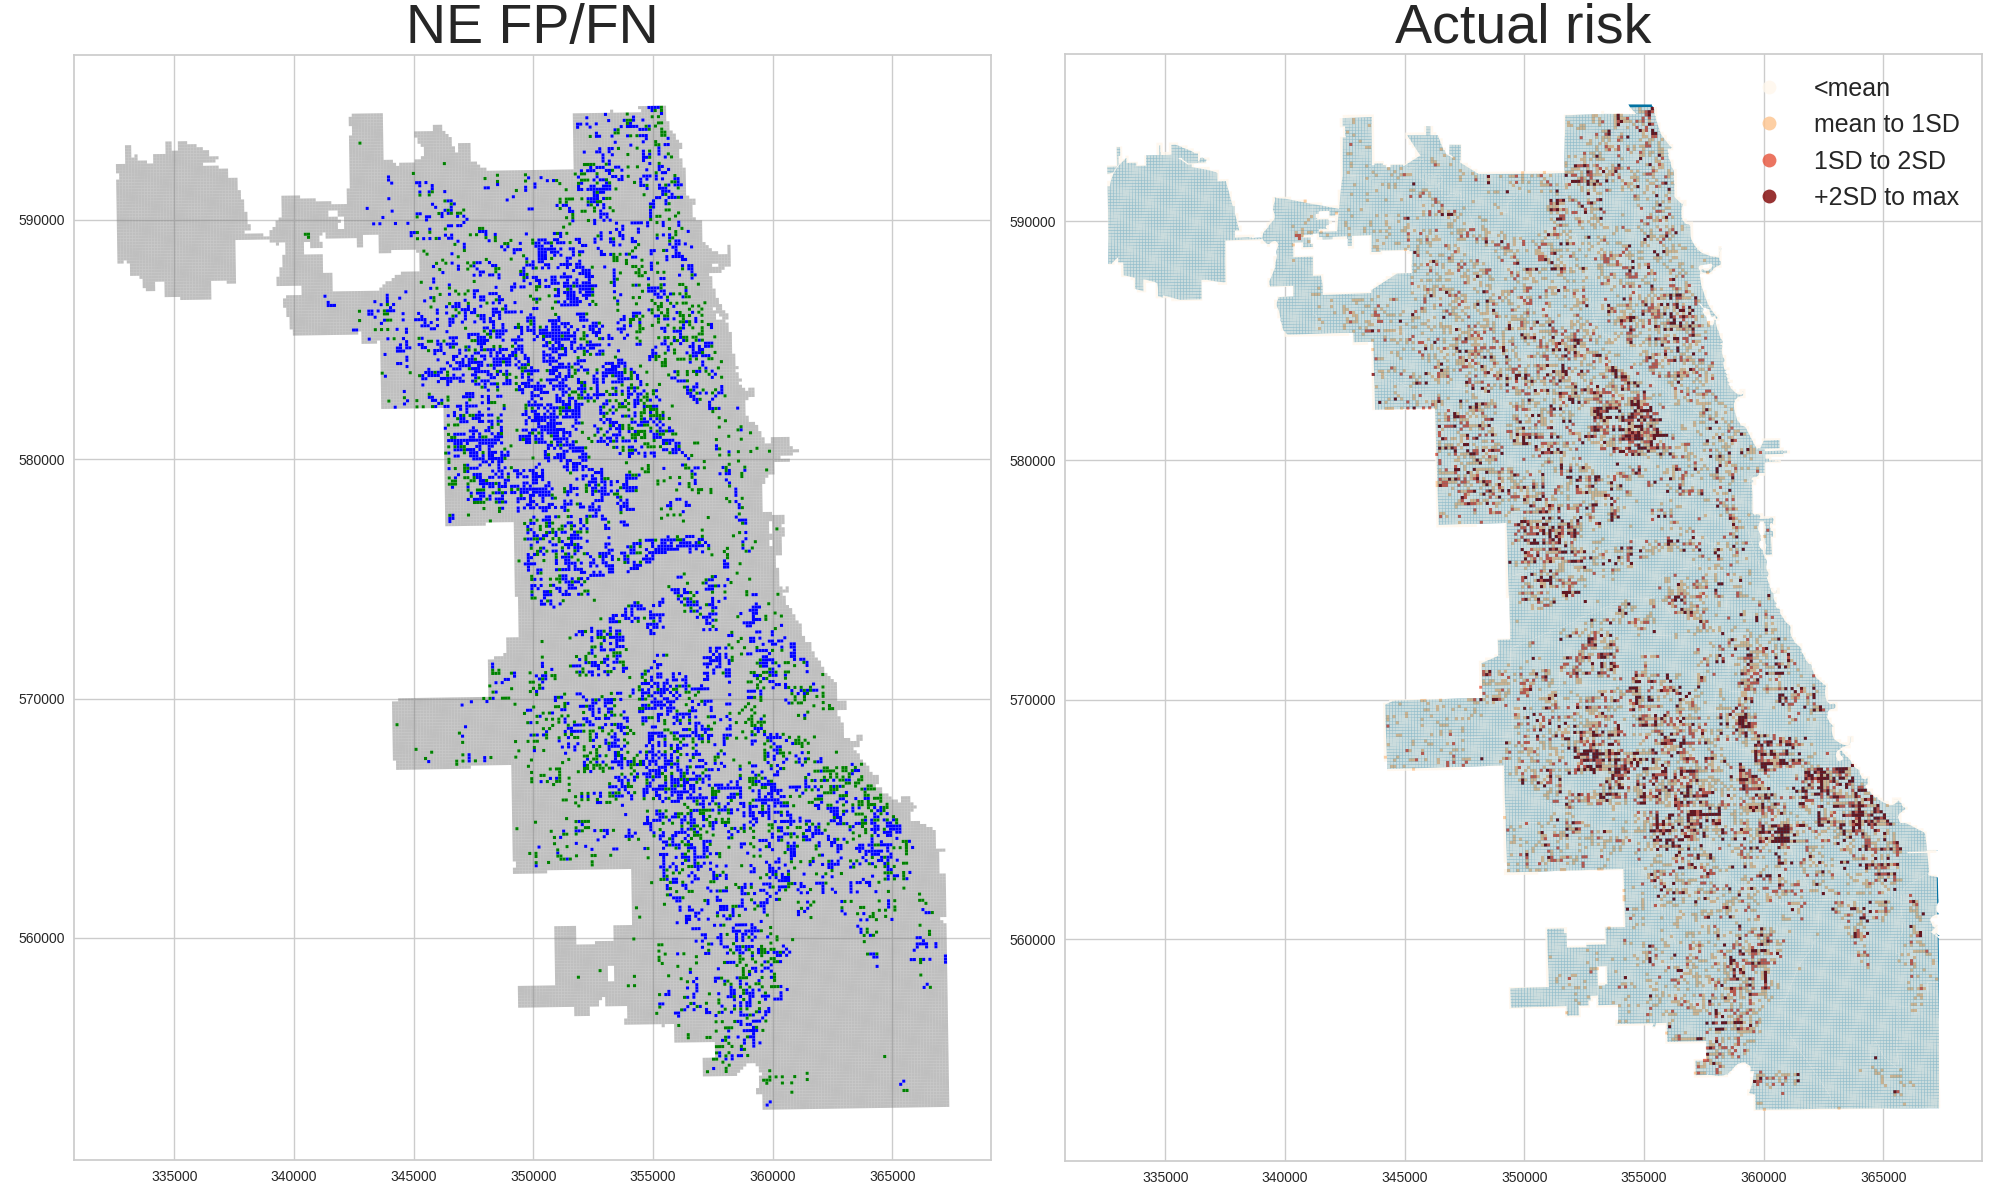
\includegraphics[scale=0.25]{./non-crime-timeseries-fig/NE_fnp.png}
%   \caption{左:NEのFPFN 右:実際のリスクマップ}
%   \label{fig:non-crime-timeseries-ne-fnp}
% \end{figure}

% \begin{figure}
%   \centering % 図を中央寄せにする
%   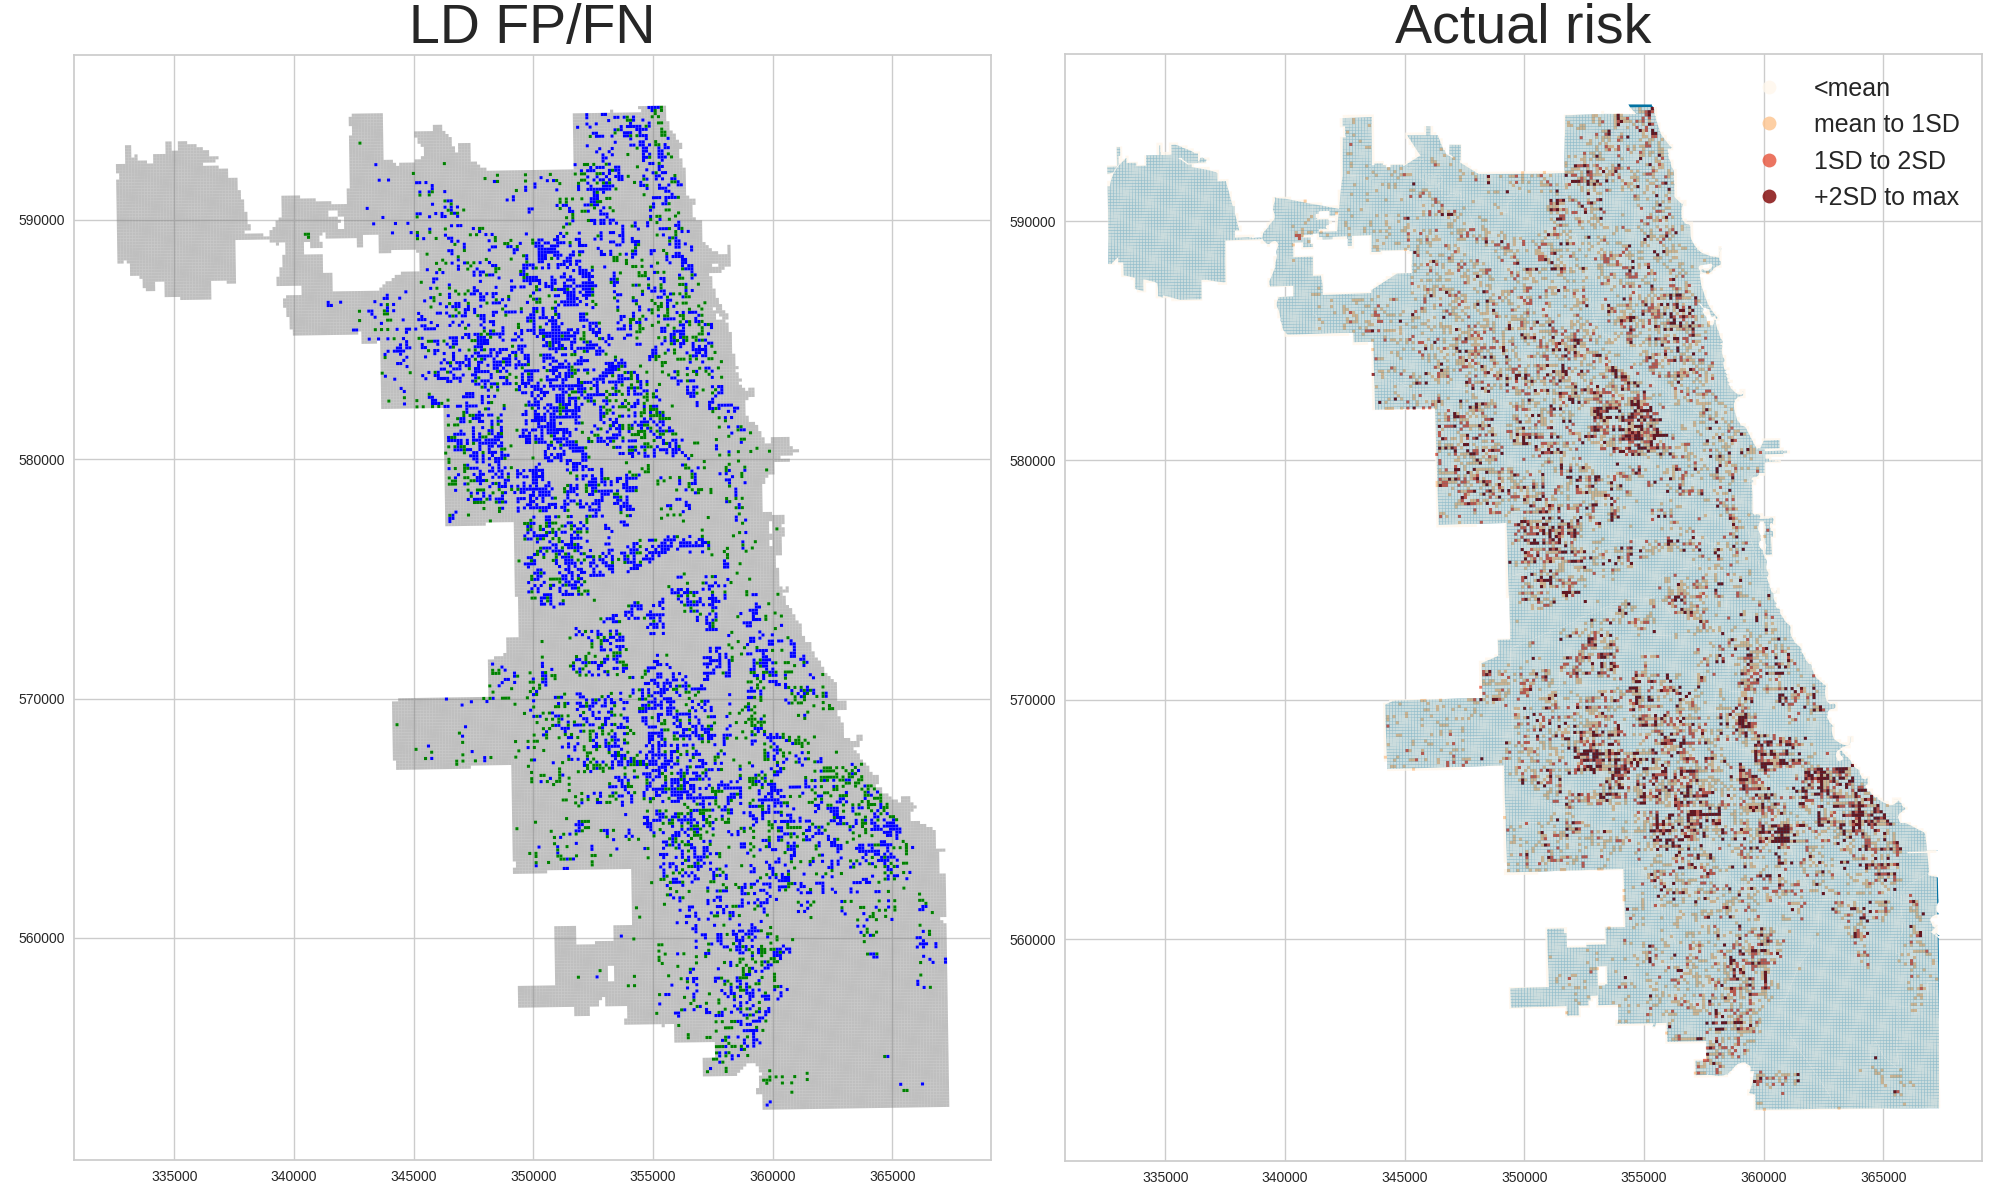
\includegraphics[scale=0.25]{./non-crime-timeseries-fig/LD_fnp.png}
%   \caption{左:LDのFPFN 右:実際のリスクマップ}
%   \label{fig:non-crime-timeseries-ld-fnp}
% \end{figure}

% \begin{figure}
%   \centering % 図を中央寄せにする
%   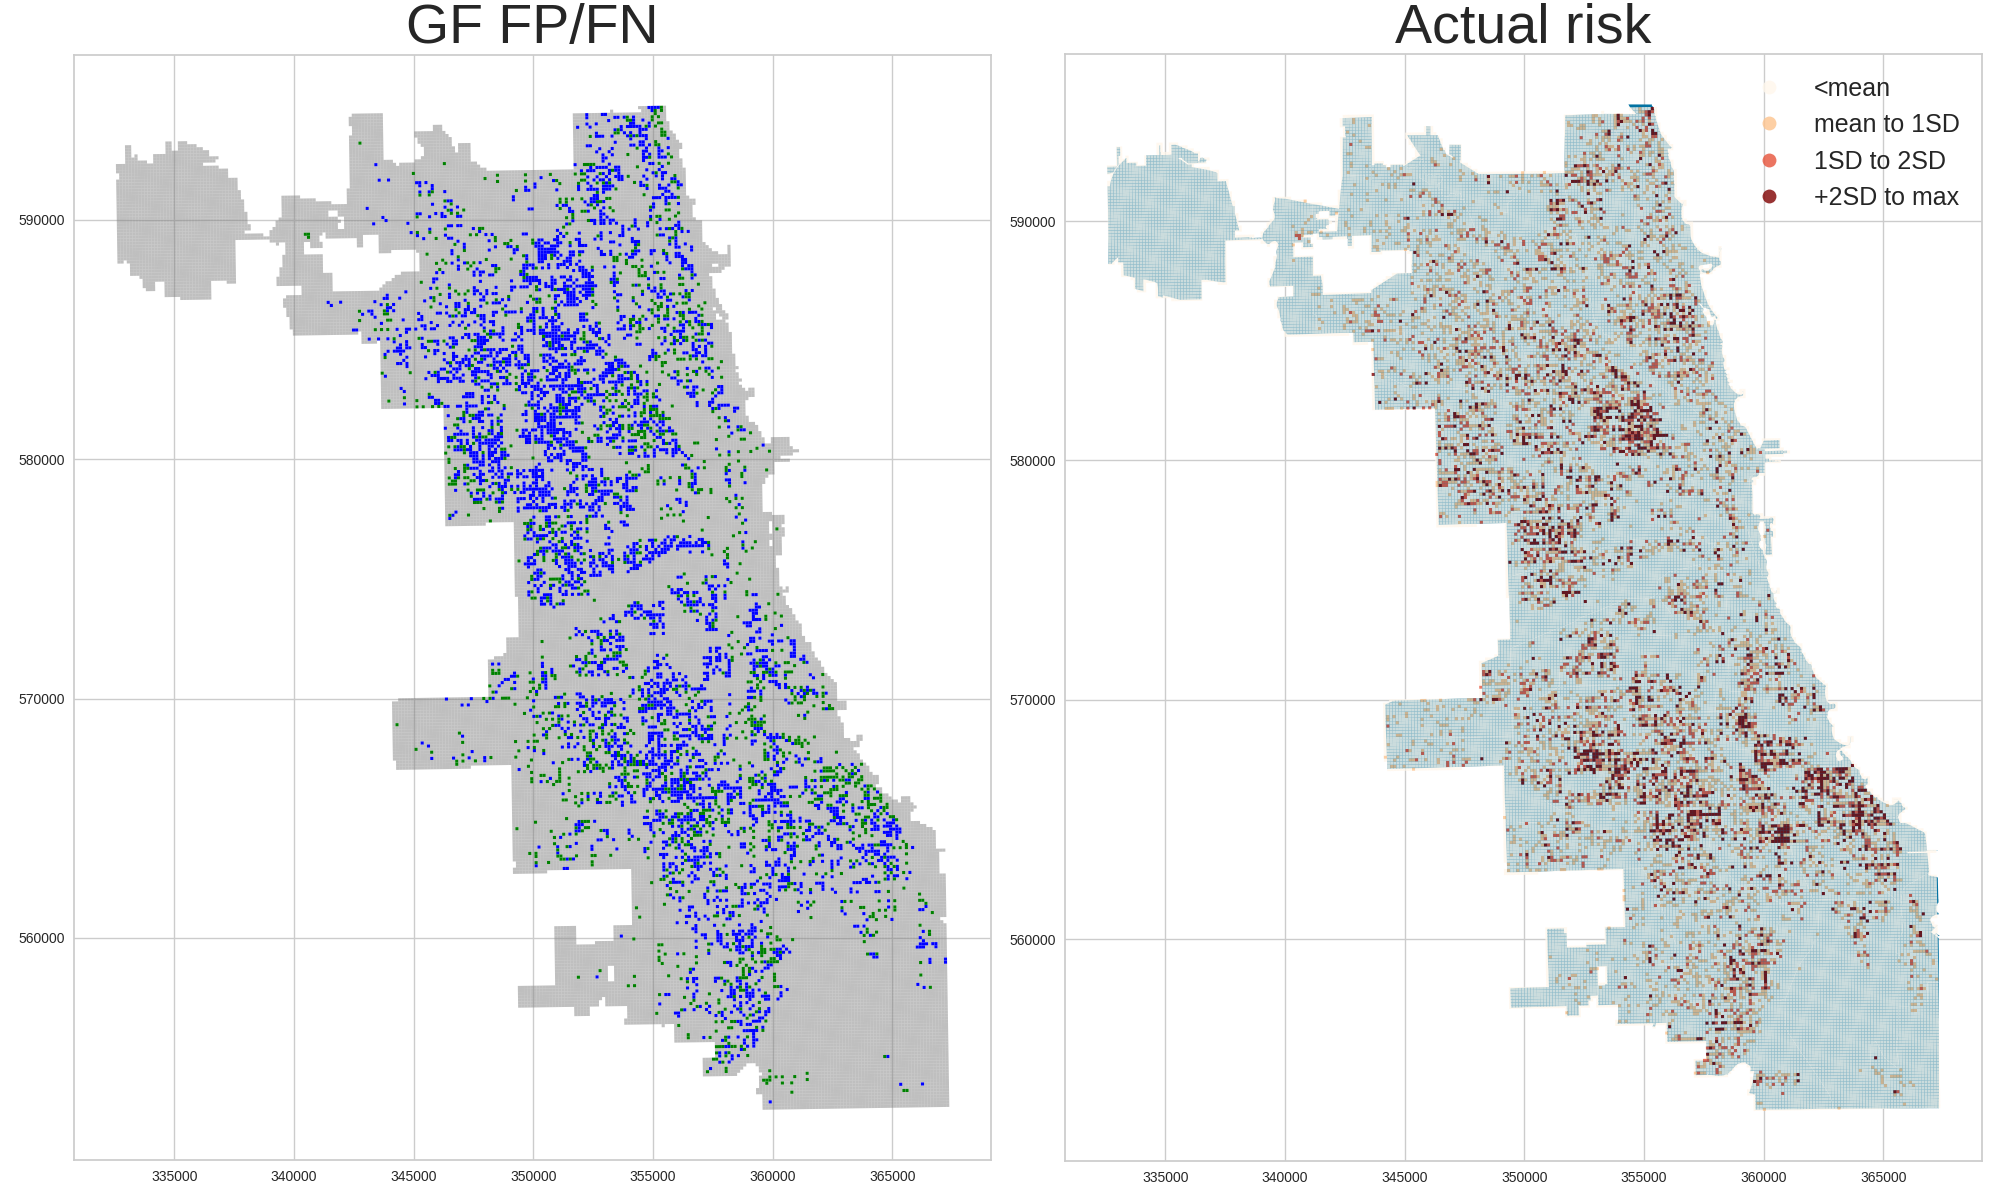
\includegraphics[scale=0.25]{./non-crime-timeseries-fig/GF_fnp.png}
%   \caption{左:GFのFPFN 右:実際のリスクマップ}
%   \label{fig:non-crime-timeseries-gf-fnp}
% \end{figure}

% \begin{figure}
%   \centering % 図を中央寄せにする
%   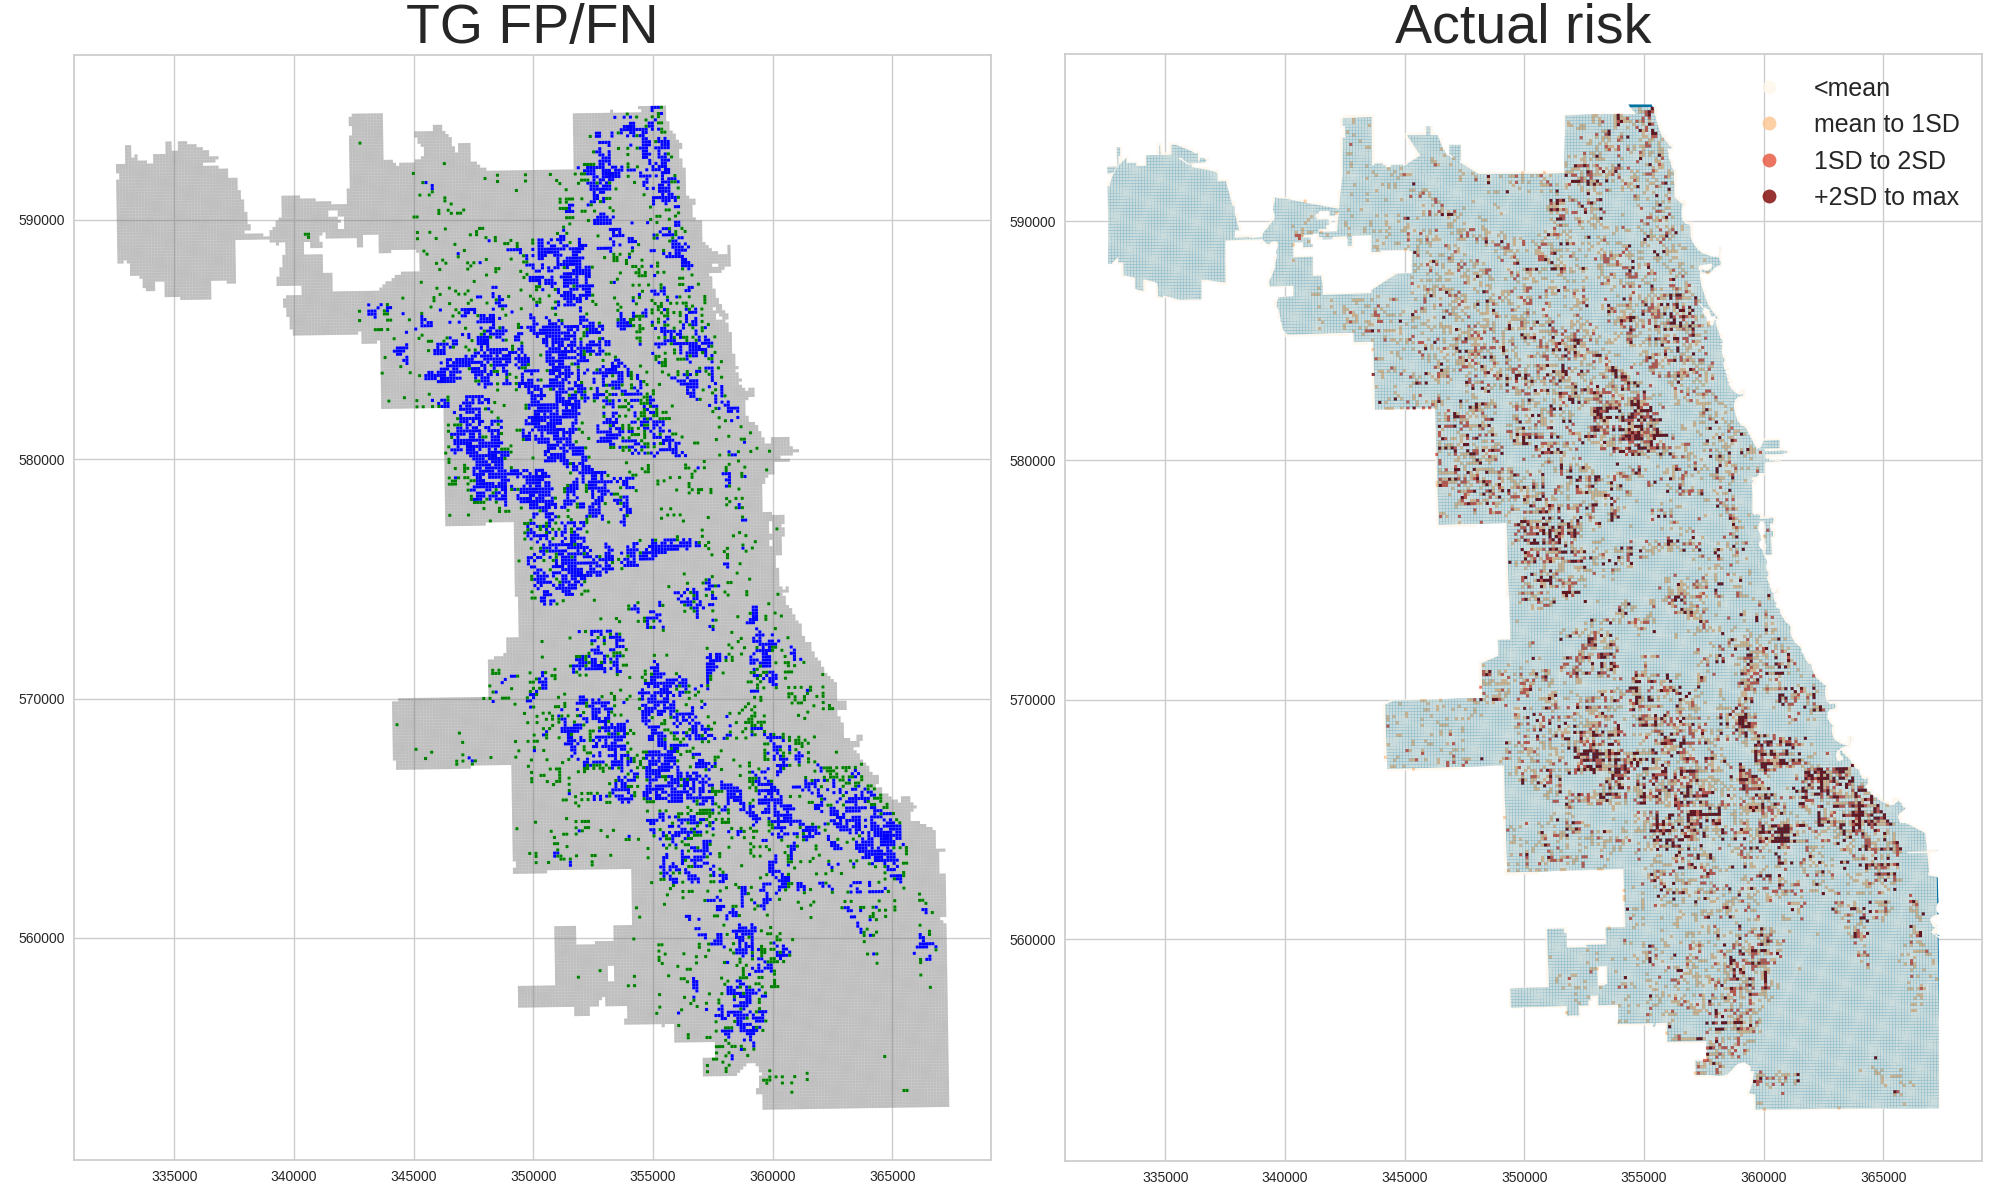
\includegraphics[scale=0.25]{./non-crime-timeseries-fig/TG_fnp.png}
%   \caption{左:TGのFPFN 右:実際のリスクマップ}
%   \label{fig:non-crime-timeseries-tg-fnp}
% \end{figure}

% \begin{figure}
%   \centering % 図を中央寄せにする
%   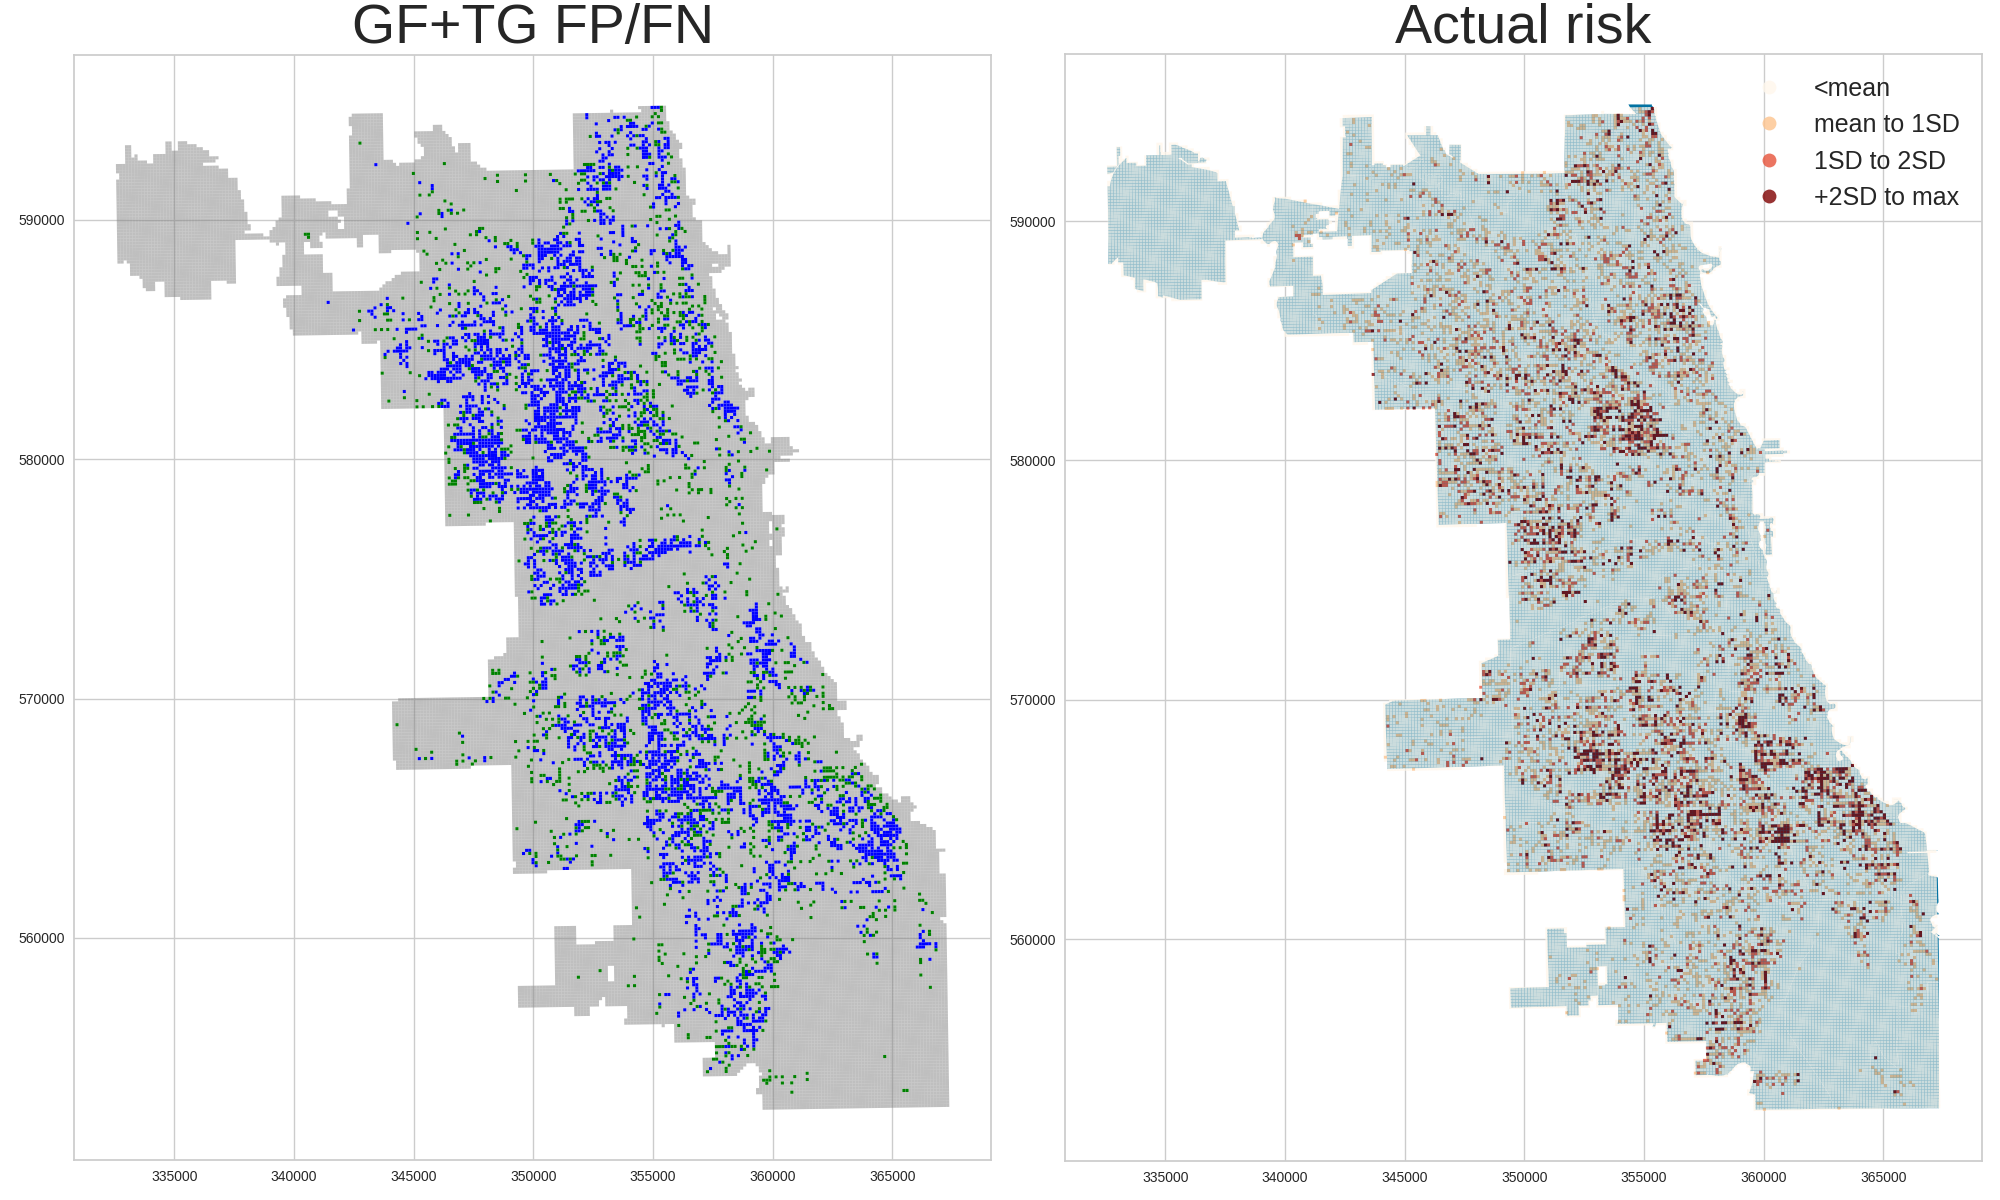
\includegraphics[scale=0.25]{./non-crime-timeseries-fig/GF+TG_fnp.png}
%   \caption{左:GF+TGのFPFN 右:実際のリスクマップ}
%   \label{fig:non-crime-timeseries-gf-tg-fnp}
% \end{figure}
% %------------------------------------------
% % ROC curve
% %------------------------------------------
% また,各モデルのROC曲線を図\ref{fig:non-crime-timeseries-roc}に示した.

% \begin{figure}
%   \centering % 図を中央寄せにする
%   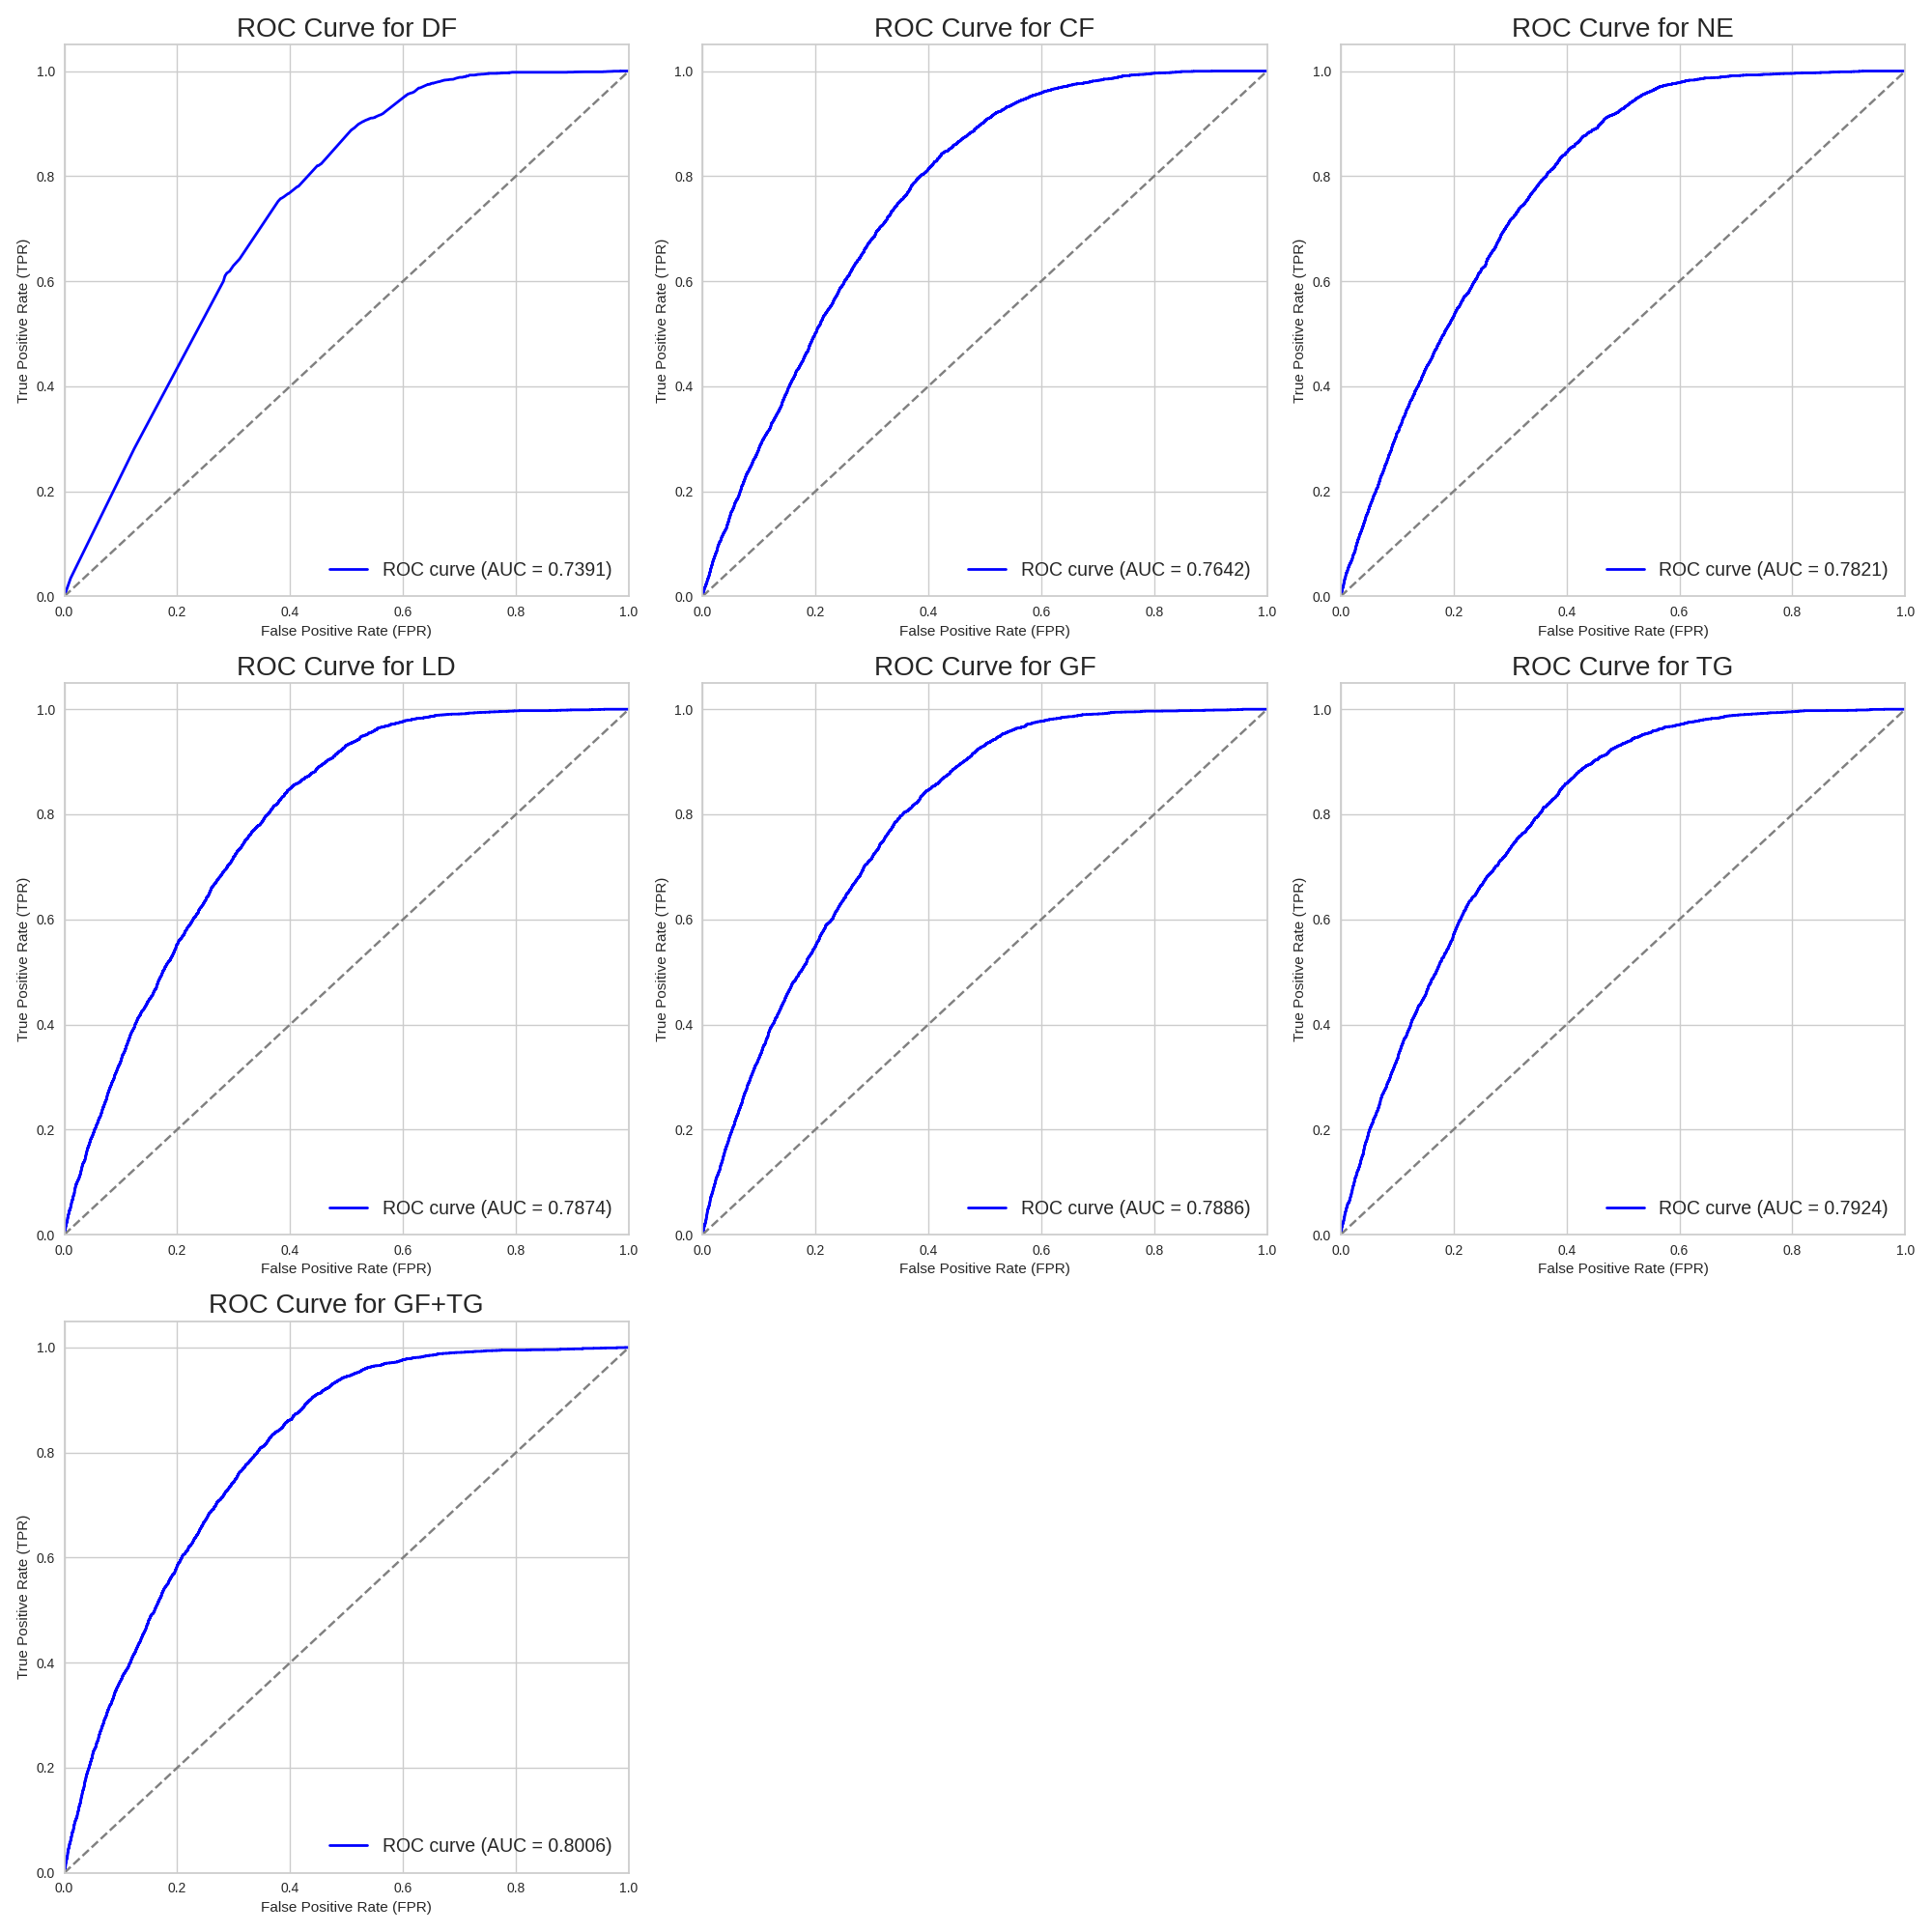
\includegraphics[scale=0.25]{./non-crime-timeseries-fig/roc_auc.png}
%   \caption{ROC曲線}
%   \label{fig:non-crime-timeseries-roc}
% \end{figure}
%------------------------------------------
% table
%------------------------------------------
各モデルの予測精度を精度指標を基に比較した結果を表\ref{tb:fig:non-crime-timeseries-index}にまとめる.
最も的中率が高いモデルはDFであるが,これは偽陽性を評価できていないのでPAIとAUCに注目する.
PAIは,DFとCFの比較から特徴量を連続化すると大きく改善し,
犯罪特徴量を追加する(CI)と更に改善することが確認できた.
またAUCは,CF・CIで同等の改善が確認できた.
% また,距離特徴量を変換するNE,LD,GF,TGではCFより改善がみられ,
% GF+TGが最もPAIが高くなった.
% AUCについて注目すると,DFとCFを比較すると精度の改善がみられた.
% LD,GF,TGでは同等の精度の改善が確認され,
% PAIと同様にGF+TGが最もAUCが高くなった.

また,DFとCIのAUC値の有意差を評価するためにDeLong検定\cite{DeLong}を実施した結果,
$p<0.001$となり,両者のAUCに統計的に有意な差があることが確認できた.

\begin{table}[htbp]
  \centering
  \caption{各モデル間の精度比較}
  \begin{tabular}{l|r||r|r}
  \hline

  モデル & DF & CF & \cfsq \\  \hline\hline
  的中率 & \bf{57.2} & 30.2 & 31.3  \\ 
  PAI & 1.84 & 2.18 & \bf{2.29} \\ 
  AUC & 0.74 & \bf{0.76} & \bf{0.76} \\ \hline
  


  \end{tabular}
  \label{tb:fig:non-crime-timeseries-index}
\end{table}

\FloatBarrier
%------------------------------------

%----------------------------------------------------------------------------
\section{おわりに}
%----------------------------------------------------------------------------
本研究で提案した連続型特徴量は,従来手法で確認されたリスクマップの空間相関を削減でき,
さらに従来手法を上回る予測精度を得た。
犯罪予測の文脈では,特徴量構成法の改善は一般的ではないが,
RTMにおいては予測精度の向上と空間相関の削減につながることが確認できた。

犯罪発生情報をRTMに取り入れることは,RTMを導入するモチベーションから離れてしまうが,
犯罪予測モデルとしては,他犯罪種の発生情報を予測に取り入れる試みが
既存のRTMを上回る予測精度を得ることが確認できた。

また従来手法によるRTMのアルゴリズムを簡略化して再実装することにより,
製品版RTMを利用するだけでは至らなかった改善を実施することができた。


\begin{thebibliography}{99}
% \bibitem[Knuth 84]{texbook}
%  Knuth,~D.~E.: The \TeX{}book, Addison-Wesley (1984),
%   (邦訳~: \TeX{}ブック, 斎藤 信男 監修, 鷺谷 好輝 訳,
%   アスキー出版局 (1992)).
% \bibitem[Lamport 86]{latexブック}
% Leslie,~L: \LaTeX{}: {A} Document Preparation System (Updated for
%   \LaTeX{}2$\varepsilon$), Addison-Wesley, 2nd edition (1998)
%   (邦訳~: 文書処理システム \LaTeX{}2$\varepsilon$,
%   阿瀬 はる美 訳, ピアソン・エデュケーション, (1999)).
\begin{thebibliography}{}

  \bibitem[Bishop 07]{bishop}
  Bishop,~C.~M.: {\em Pattern Recognition and Machine Learning (Information Science and Statistics)}, Springer, 1 edition (2007)
  
  \bibitem[Caplan 15]{caplan2015risk}
  Caplan,~J.~M.et al.: Risk terrain modeling for spatial risk assessment, {\em Cityscape}, Vol.~17, No.~1, pp. 7--16 (2015)
  
  \bibitem[CDPH 24]{ChicagoDataPortal}
  Chicago Department of Public Health. (2024), \url{https://data.cityofchicago.org/}
  
  \bibitem[Chainey 08]{chainey2008utility}
  Chainey,~S. et al.: The utility of hotspot mapping for predicting spatial patterns of crime, {\em Security journal}, Vol.~21, pp. 4--28 (2008)
  
  \bibitem[DeLong 88]{DeLong}
  DeLong,~E.~R., et al.: Comparing the Areas under Two or More Correlated Receiver Operating Characteristic Curves: A Nonparametric Approach, {\em Biometrics}, Vol.~44, No.~3, pp. 837--845 (1988)
  
  \bibitem[Hastie 01]{esl}
  Hastie,~T., et al.: {\em The Elements of Statistical Learning}, Springer Series in Statistics, Springer New York Inc., New York, NY, USA (2001)
  
  \bibitem[Hilbe 11]{Hilbe_2011}
  Hilbe,~J.~M.: {\em Negative Binomial Regression}, Cambridge University Press, 2 edition (2011)

  \bibitem[Yeo 00]{yeo}
  I. Yeo , R. Johnson: A new family of power transformations to improve normality or symmetry {\em Biometrika}, vol. 87, pp. 954--959, (2000)

  \bibitem[James 23]{islp}
  James,~G., et al.: {\em An Introduction to Statistical Learning with Applications in Python}, Springer Texts in Statistics, Springer, Cham (2023)
  
  \bibitem[Jordahl 20]{geopandas}
  Jordahl,~K., et al.: geopandas/geopandas: v0.8.1 (2020)
  
  \bibitem[Joshi 20]{joshi2020considerationsdevelopingpredictivemodels}
  Joshi,~C. et al.: Considerations for developing predictive models of crime and new methods for measuring their accuracy (2020)
  
  \bibitem[Nelder 72]{poisson}
  Nelder,~J.~A., Wedderburn,~R.~W.~M.: Generalized Linear Models, {\em Journal of the Royal Statistical Society. Series A (General)}, Vol. 135, No.~3, pp. 370--384 (1972)
  
  \bibitem[Pedregosa 11]{scikit-learn}
  Pedregosa,~F. et al.: Scikit-learn: Machine Learning in {P}ython, {\em Journal of Machine Learning Research}, Vol.~12, pp. 2825--2830 (2011)
  
  \bibitem[Tibshirani 96]{Lasso}
  Tibshirani,~R.: Regression shrinkage and selection via the lasso, {\em Journal of the Royal Statistical Society Series B: Statistical Methodology}, Vol.~58, No.~1, pp. 267--288 (1996)
  
  \bibitem[守山 22]{犯罪予測}
  守山正:犯罪予測 : AIによる分析, 成文堂 (2022)
  
  \bibitem[大山 17]{地理的犯罪予測研究の潮流}
  大山智也 et al.:地理的犯罪予測研究の潮流, GIS-理論と応用, Vol.~25, No.~1, pp. 33--43 (2017)
  
  \bibitem[大山 20]{大山智也2020日本}
  大山智也:日本における地理的犯罪予測手法の開発に関する研究 (2020)
  
  \end{thebibliography}
  
% \bibitem[Caplan 15]{caplan2015risk}
% Joel~M Caplan, Leslie~W Kennedy, Jeremy~D Barnum, and Eric~L Piza.
% \newblock Risk terrain modeling for spatial risk assessment.
% \newblock \emph{Cityscape}, 17\penalty0 (1):\penalty0 7--16, 2015.

% \bibitem[CDPH 24]{ChicagoDataPortal}
% Chicago~Department of~Public~Health, 2024.
% \newblock \url{https://data.cityofchicago.org/}.

% \bibitem[守山 22]{犯罪予測}
% 正~守山.
% \newblock \emph{犯罪予測 : AIによる分析}.
% \newblock 成文堂, 2022.
% \newblock URL \url{https://ci.nii.ac.jp/ncid/BC14107703}.
\end{thebibliography}


%%
